\documentclass[a4paper, 12pt]{article}

%%%%%%%%%%%%
% Packages %
%%%%%%%%%%%%

\usepackage[english]{babel}
\usepackage{packages/sleek}
\usepackage{csvsimple}
\usepackage{booktabs} % for nicer table rules
\usepackage{float}
\usepackage{listings}
\usepackage{xcolor}
\usepackage{inconsolata}  % Nicer monospace font
\usepackage{graphicx} % For including images
\usepackage{subcaption}  % in preamble
\usepackage{enumitem}

\usepackage{tikz}
\usetikzlibrary{arrows.meta, positioning, shapes.geometric}

\lstset{
  basicstyle=\ttfamily\small,        % Smaller monospaced font
  frame=single,                        % No box frame=none
  breaklines=true,                   % Automatic line breaks
  columns=fullflexible,              % Better spacing
  showstringspaces=false,            % Don't show spaces in strings
  tabsize=2,                         % Tabs = 2 spaces
  numbers=left,                      % Line numbers on the left
  numberstyle=\tiny\color{gray},     % Smaller line number style
  captionpos=b,                      % Caption below the code
  keywordstyle=\color{blue},         % Keywords in blue
  commentstyle=\color{gray},         % Comments in gray
  stringstyle=\color{orange},        % Strings in orange
  numbers=none, % No line numbers
}

% Custom style for code listings
\lstdefinestyle{plain}{
    basicstyle=\ttfamily\small,
    frame=none,
    breaklines=true,
    columns=fullflexible,
    showstringspaces=false,
    tabsize=2,
    numbers=none,
}
\lstset{style=plain}


\addbibresource{./resources/bib/references.bib}


\newcommand{\projectTitle}{YouBot Project}
\newcommand{\projectSubtitle}{Redeployment and quantitative assessment of the KUKA YouBot}
\newcommand{\authorName}{Aditya Agrawal}
\newcommand{\advisorName}{assistant professor Tomasz Kucner}
\newcommand{\supervisorName}{senior university lecturer Salu Ylirisku}
\newcommand{\courseName}{ELEC-C0302 Final Project in Digital Systems and Design}
\newcommand{\universityName}{Aalto University}


\newcommand{\commentout}[1]{}
\newif\ifshowadi
\showaditrue% Set to \showaditrue to display comments on extending thesis

\newcommand{\adi}[1]{\ifshowadi\textcolor{red}{#1}\fi}

\newif\ifshownotes
\shownotestrue% Set to \shownotestrue to display notes

\newcommand{\notes}[1]{\ifshownotes\textcolor{blue}{#1}\fi}

\newcommand{\code}[1]{\texttt{\detokenize{#1}}}




%%%%%%%%%%%%
% Document %
%%%%%%%%%%%%

\begin{document}

%%%%%%%%%%%%%%
% Title-page %
%%%%%%%%%%%%%%
    \begin{titlepage}
        \raggedright
        % Define variables for title page
        

        \vspace*{2cm}

        {\Huge \textbf{\projectTitle}}\\[0.5cm]
        {\Large \projectSubtitle}\\[2cm]

        \textbf{Author:} \authorName\\[0.3cm]
        \textbf{Advisor:} \advisorName\\[0.3cm]
        \textbf{Supervisor:} \supervisorName\\[2cm]

        \courseName \\
        \universityName\\[0.5cm]
        \today

        \vfill
    \end{titlepage}
    \setcounter{tocdepth}{2} % Only show sections and subsections in TOC
    \romantableofcontents

    \commentout{\section{Ideas \& Drafts (NOT ON FINAL REPORT)}
    structure: 
    My work
    reflection
    appendix: user manual

    things I did i want to add:
    - add in the initial project plan
    - add in the initial state of everything
    - known documentation

    - libfreenect and kinect camera
    - communication with onboard computer
    - enabling it to initially move through provided demos
    - utilising ROS1-ROS2 bridge (fail)
    - fixing the battery up 
    - writing my own programs to move the bot 
    
    - how did my goals change with time?
    - project management brief overview
    Teach and repeat background:
    https://furgalep.github.io/bib/mcmanus_icra12.pdf
    https://www.sciencedirect.com/science/article/pii/S0921889020304176
    https://arxiv.org/pdf/2309.15405
    https://clearpathrobotics.com/blog/2018/07/visual-teach-and-repeat-closer-look-part-1/}

    
    
    \section{Introduction}

    \subsection{Motivation}

    \notes{draft \#2}

    In the rapidly evolving field of robotics, expensive hardware platforms often become obsolete quickly. This is not purely because of physical wear and tear or a lack of functionality, but also due to quick advancements in hardware, software and infrastructure. For example, artificial intelligence (AI) and related fields like Machine Learning (ML) and Deep Learning (DL) has accelerated progress within robotics, driving demand for specialised, high-performance hardware and tightly integrated software ecosystems. Consequently,older robotic platforms, despite their inherent capabilities, become less relevant and lose extended support. This furthermore could lead to increased e-waste and reduced sustainability in the robotics industry \cite{KARASTOYANOV201844}. 

    The KUKA YouBot is a prime example of this phenomenon. It was once a popular platform for research and education in robotics in the mid-2010s, but has been since discontinued and is no longer supported by the manufacturer. This mobile robot base is quite robust, compact and utilizes open-source drivers. While this platform has reduced performance and integration capabilities compared to its modern peers, it can still serve a variety of purposes for the purposes of industrial and academic research. This includes autonomous navigation, perception and human-robot interaction. Instead of discarding such platforms, we should explore avenues to extend their lifespan and utility. This would reduce e-waste and costs associated with acquiring new hardware, and thus lower the barrier to entry for research and development in robotics.
    
    This project aims to explore and demonstrate the potential of legacy robotic hardware like the KUKA YouBot within the modern robotics landscape. By repurposing such platforms in the context of its technical capabilities and applications, we can showcase the long-term viability of older platforms whilst allowing for smooth integration with other systems. 

    \subsection{Project Overview}

    This report documents the progress of redeploying the KUKA YouBot mobile base, and quantitatively assessing its capabilities in terms of navigation and odometry. 

    Section 2 details the initial state of the YouBot, including its hardware and software components, and describes the initial objectives of this project. Section 3 presents the revised technical and learning objectives of the project. Section 4 describes the system development process, covering initial configuration, battery and sensor integration, and custom script development. Section 5 explains the experimental setup for evaluating movement and odometry performance. Section 6 discusses the future potential of the YouBot for long-term research and industrial use cases, while section 7 concludes the report with a personal reflection on the project and its outcomes. The appendix includes a user manual for the YouBot, as well as relevant code files and experimental data.
    
    \pagebreak

    \section{Initial state of YouBot}

    The YouBot is a mobile robotic platform developed by German automation company KUKA \cite{KUKAYouBotFlyer}. First introduced in the early 2010s, it was primarily designed for research and educational purposes in the field of mobile robotics \cite{KUKAYouBotManual2013}. To further this purpose, a significant portion of software used on the YouBot is open-source and available on GitHub \cite{KUKAYouBotManual2013,githubYoubotOverview}.

    The YouBot typically consists of two main parts: a mobile base and a robotic arm. The mobile base is equipped with four omnidirectional mecanum wheels and motors for movement, alongside an onboard computer for processing and control. This onboard computer runs Ubuntu and ROS1, with conveniently provided drivers and wrappers, allowing for smooth software integration. The robotic arm has 5 degrees of freedom (DOF) and a two-finger gripper \cite{KUKAYouBotManual2013}, enabling it to perform a variety of tasks through the onboard computer. Since this project involves only the mobile base, we will not be discussing the arm in detail.

    The YouBot's open-source software stack and ROS compatibility provide a versatile foundation for both low-level hardware interfacing and high-level algorithm development. This robot and the attached sensor modules are thus particularly well-suited for research within mobile robotics, particularly those pertaining to navigation, perception and human-robot interaction. 

    \begin{figure}[H]
        \centering
        \begin{subfigure}[t]{0.49\linewidth}
            \centering
            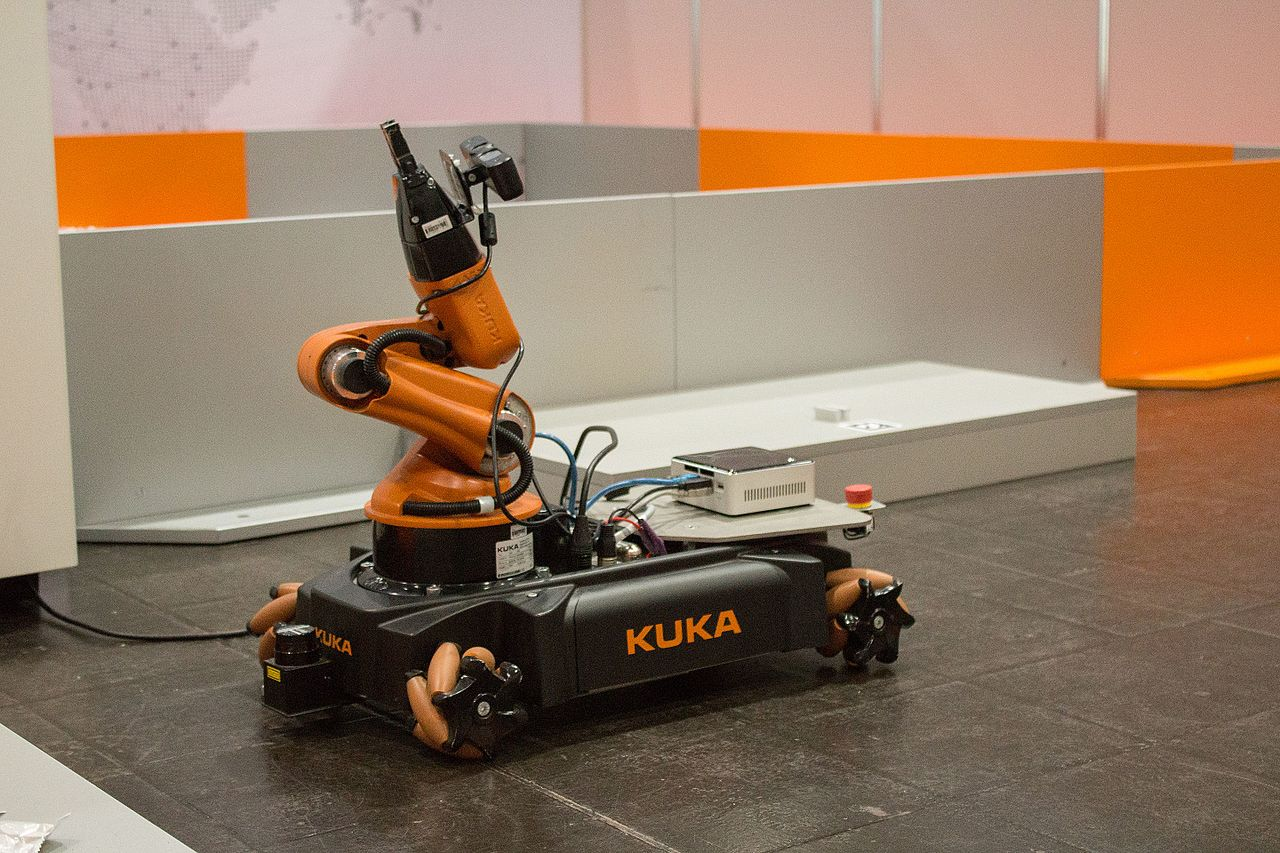
\includegraphics[width=\linewidth]{images/sec2/youbot_with_arm.png}
            \caption{The robot at RoboCup 2016 Leipzig \cite{ubahnverleih2016}.}
        \end{subfigure}
        \hfill
        \begin{subfigure}[t]{0.49\linewidth}
            \centering
            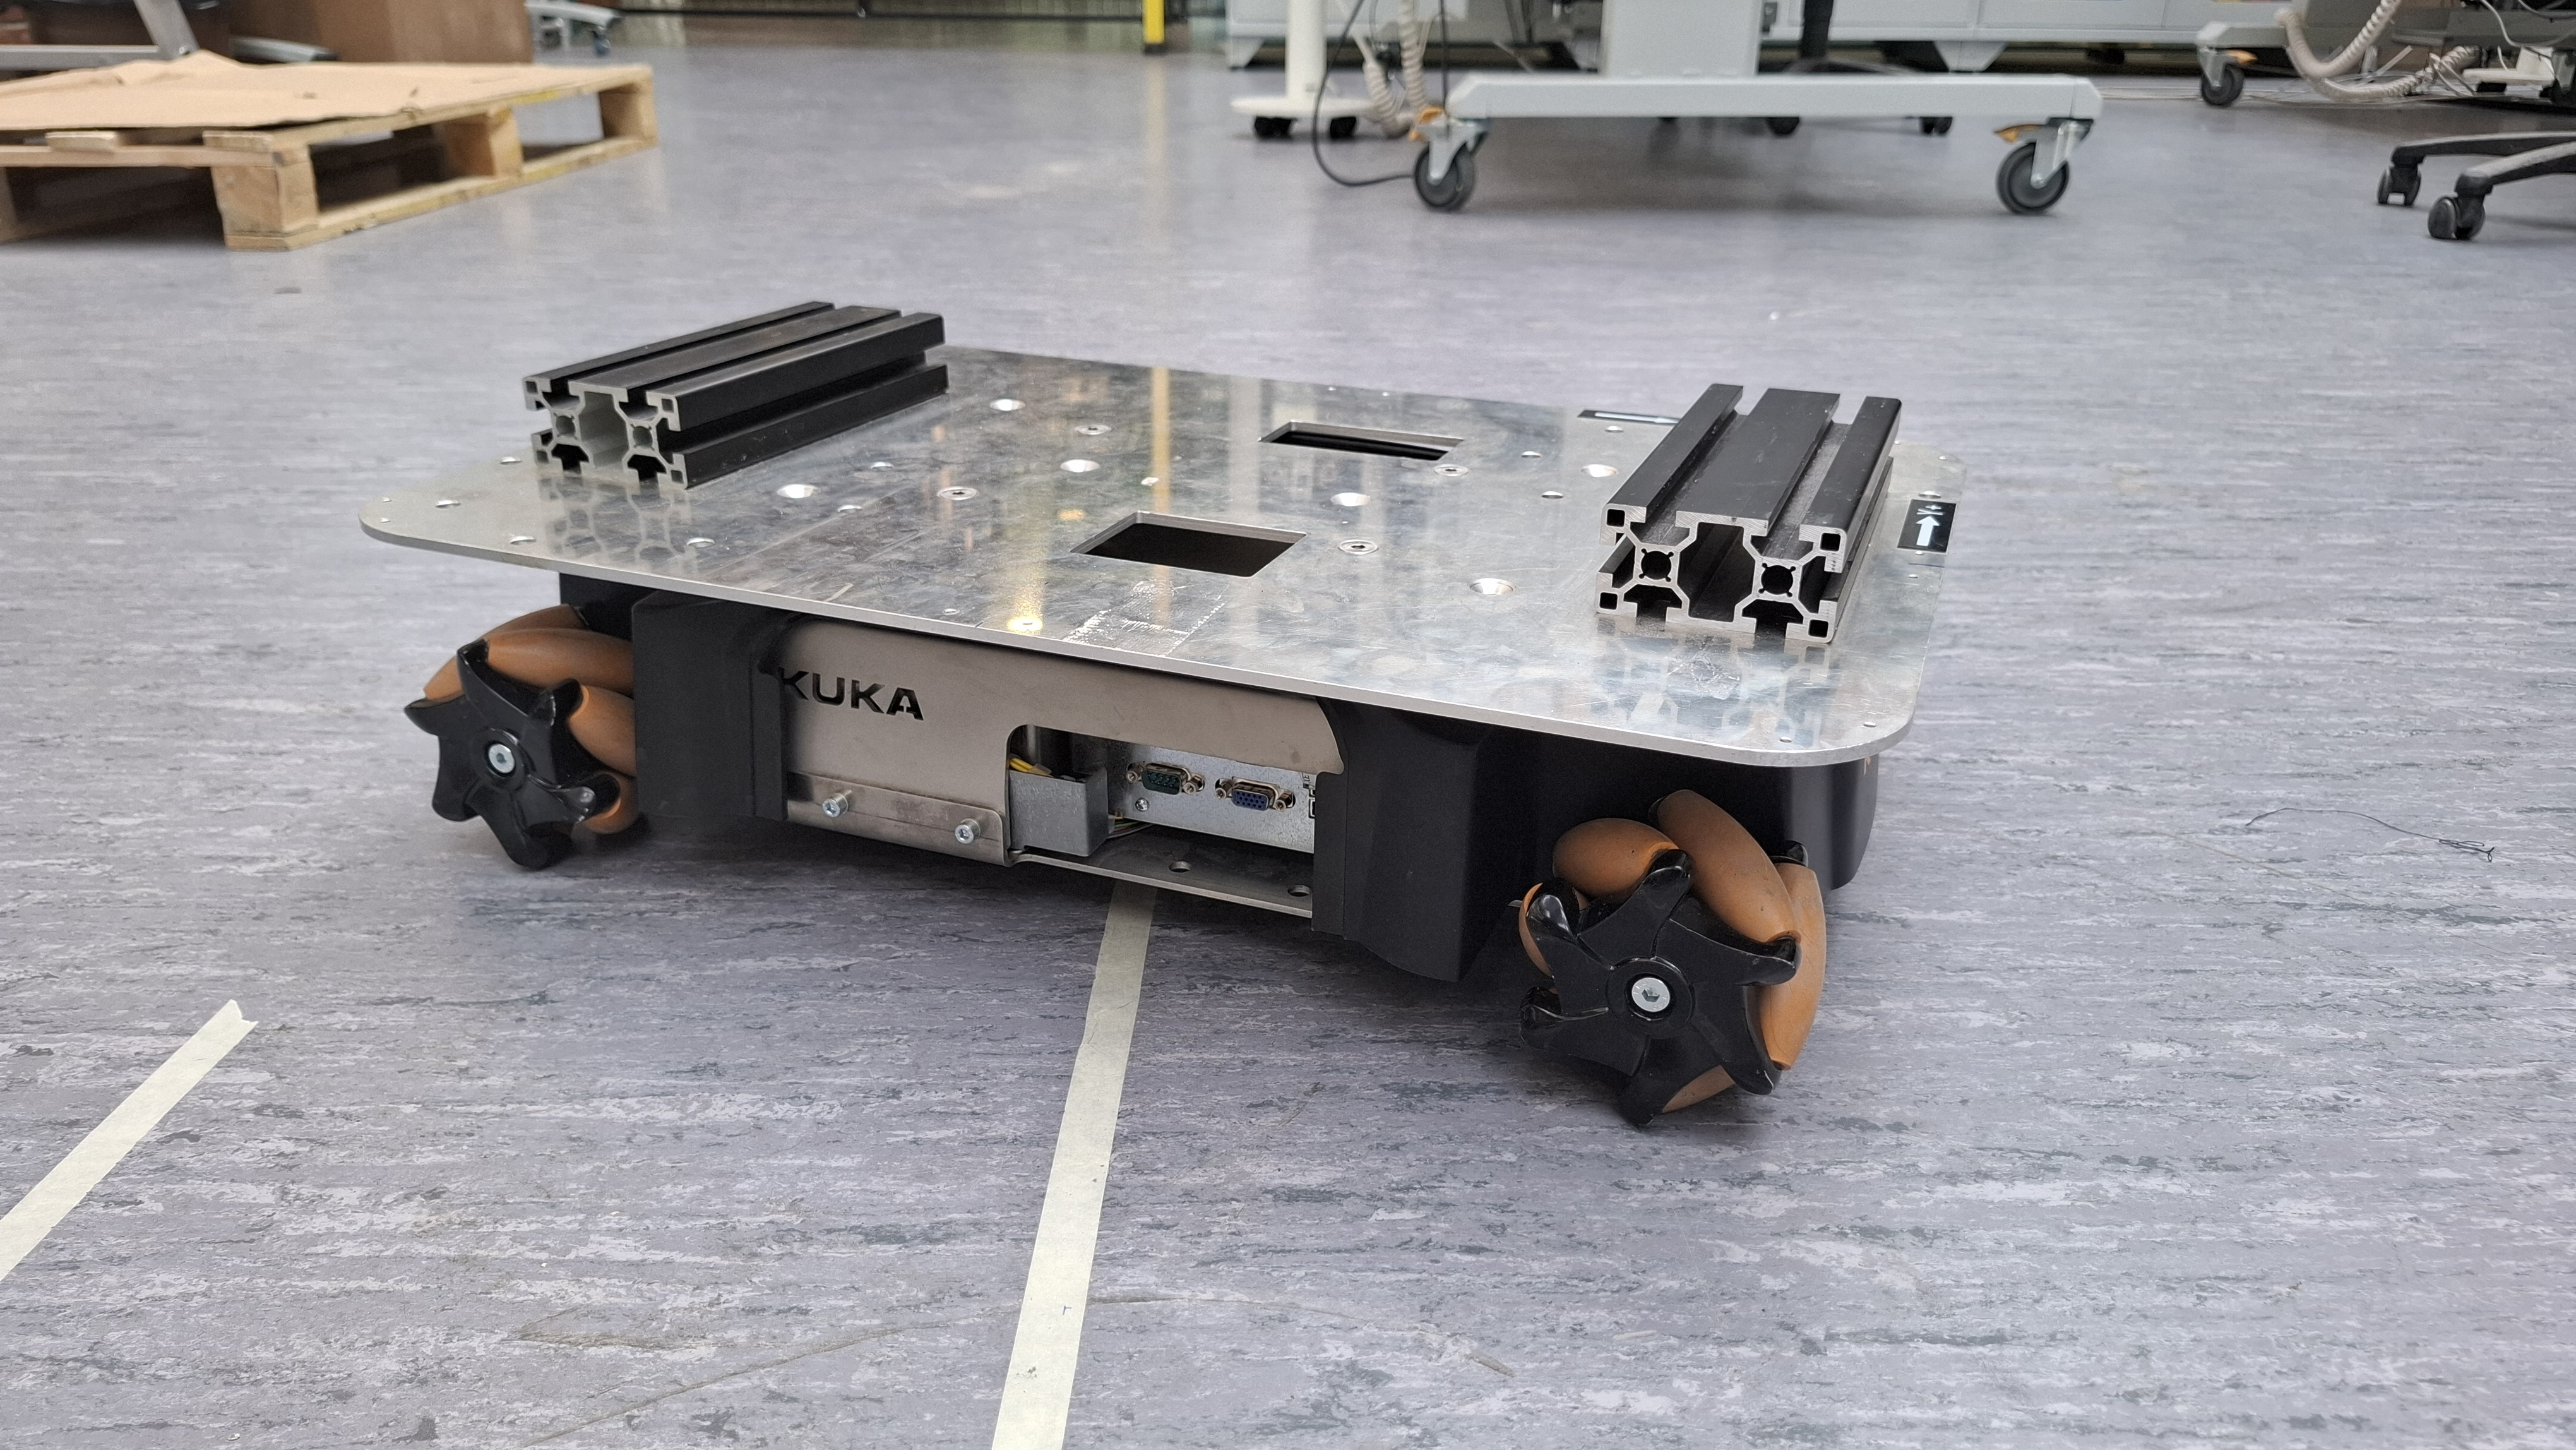
\includegraphics[width=\linewidth]{images/sec2/youbot_irl.jpg}
            \caption{The robot as used in the Aalto University Robotics Lab.}
            \label{fig:youbot-aalto}
        \end{subfigure}
        \caption{The YouBot.}
    \end{figure}

    \subsection{Onboard Computer}

    The onboard computer features a Intel Atom D510 @ 1.66GHz processor, with a 2GB DDR2 RAM and 32GB SSD hard drive. 

    The computer currently runs Ubuntu 12.04.5 LTS with ROS1 Hydro, which is a decade-old version of the operating system and the robot operating system. Given the age of the OS and ROS, compatibility with modern libraries and software is limited. Essential drivers and wrappers were already installed to enable communication with the robot's motors and sensors. These could be accessed directly through C++ programs or through ROS packages. For the purposes of this project, we have elected to focus on the latter to allow for a seamless integration with the ROS ecosystem in the future, alongside a level of standardization and ease of use.

    \subsection{Connection Interfaces}

    To interface with the onboard PC, the YouBot features panels with several connection ports. The top panel of the robot contains two EtherCAT ports for consistent real-time communication with motion-oriented systems (i.e. robotic manipulators), and a standard Ethernet port for wired interfacing with an external computer or network. Adjacent to these communication ports are a power button and a small screen that displays input voltage and ON/OFF state of the onboard PC and motors (Figure~\ref{fig:youbot-screen}). Furthermore, the right side of the robot features a panel with a VGA port for video output, as well as six USB 2.0 ports for connecting peripherals such as a keyboard, mouse, or wireless adapter (Figure~\ref{fig:youbot-usb}). 

    \begin{figure}[H]
        \centering
        % Row 2
        \begin{subfigure}[t]{0.49\linewidth}
            \centering
            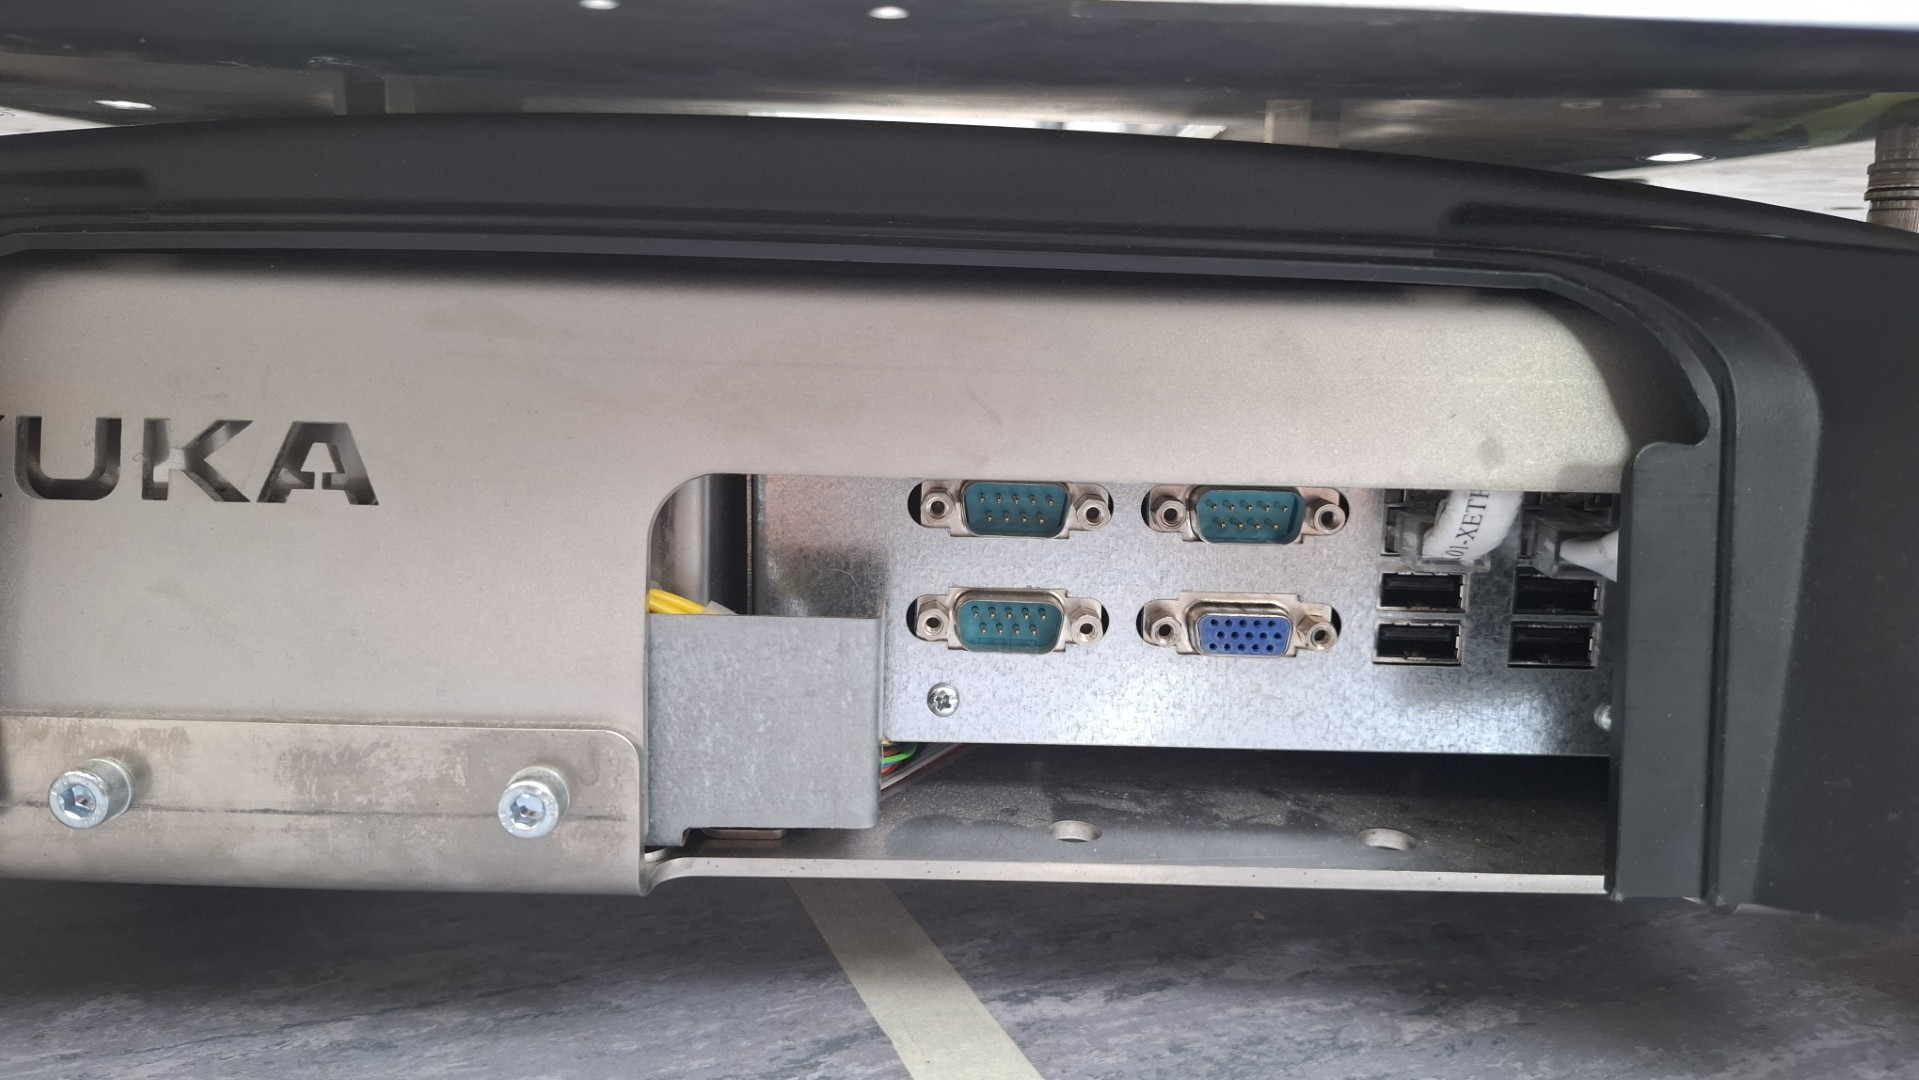
\includegraphics[width=\linewidth]{images/sec2/youbot_usb_ports.jpg}
            \caption{The right side of the robot, showing the VGA and USB ports.}
            \label{fig:youbot-usb}
        \end{subfigure}
        \hfill
        \begin{subfigure}[t]{0.49\linewidth}
            \centering
            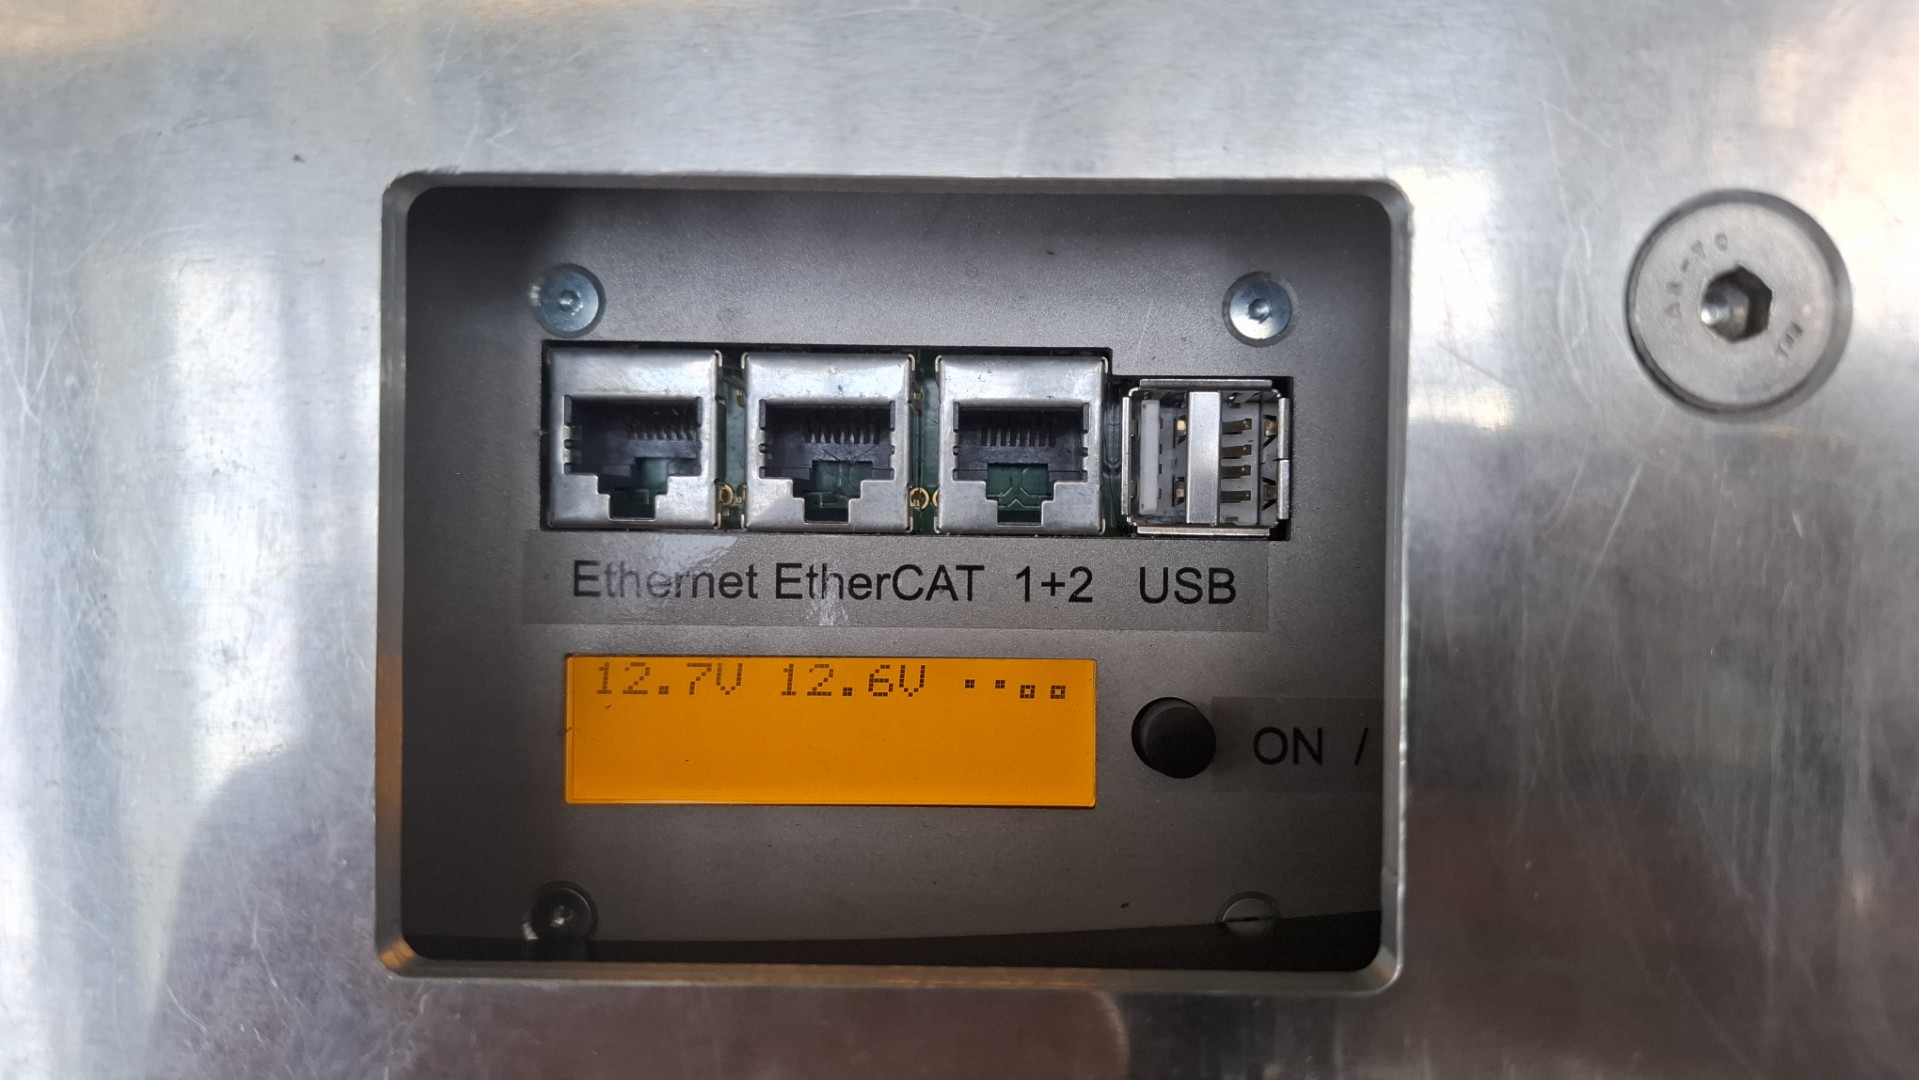
\includegraphics[width=\linewidth]{images/sec2/youbot_screen.jpg}
            \caption{The onboard computer screen, alongside the power button and EtherCAT/Ethernet ports.}
            \label{fig:youbot-screen}
        \end{subfigure}

        \caption{Connection points on the YouBot.}
        \label{fig:youbot-connections}
    \end{figure}


    \subsection{Power}

    The YouBot is powered by a 24V power supply, which can be connected through a 3-pin XLR connector located on the top panel of the robot. Additionally, the base includes two 24V 3-pin XLR output ports, which are intended for powering external components such as robotic manipulators or sensors (Figure~\ref{fig:youbot-power}).

    \begin{figure}[H]
        \centering
        \begin{subfigure}[t]{0.49\linewidth}
            \centering
            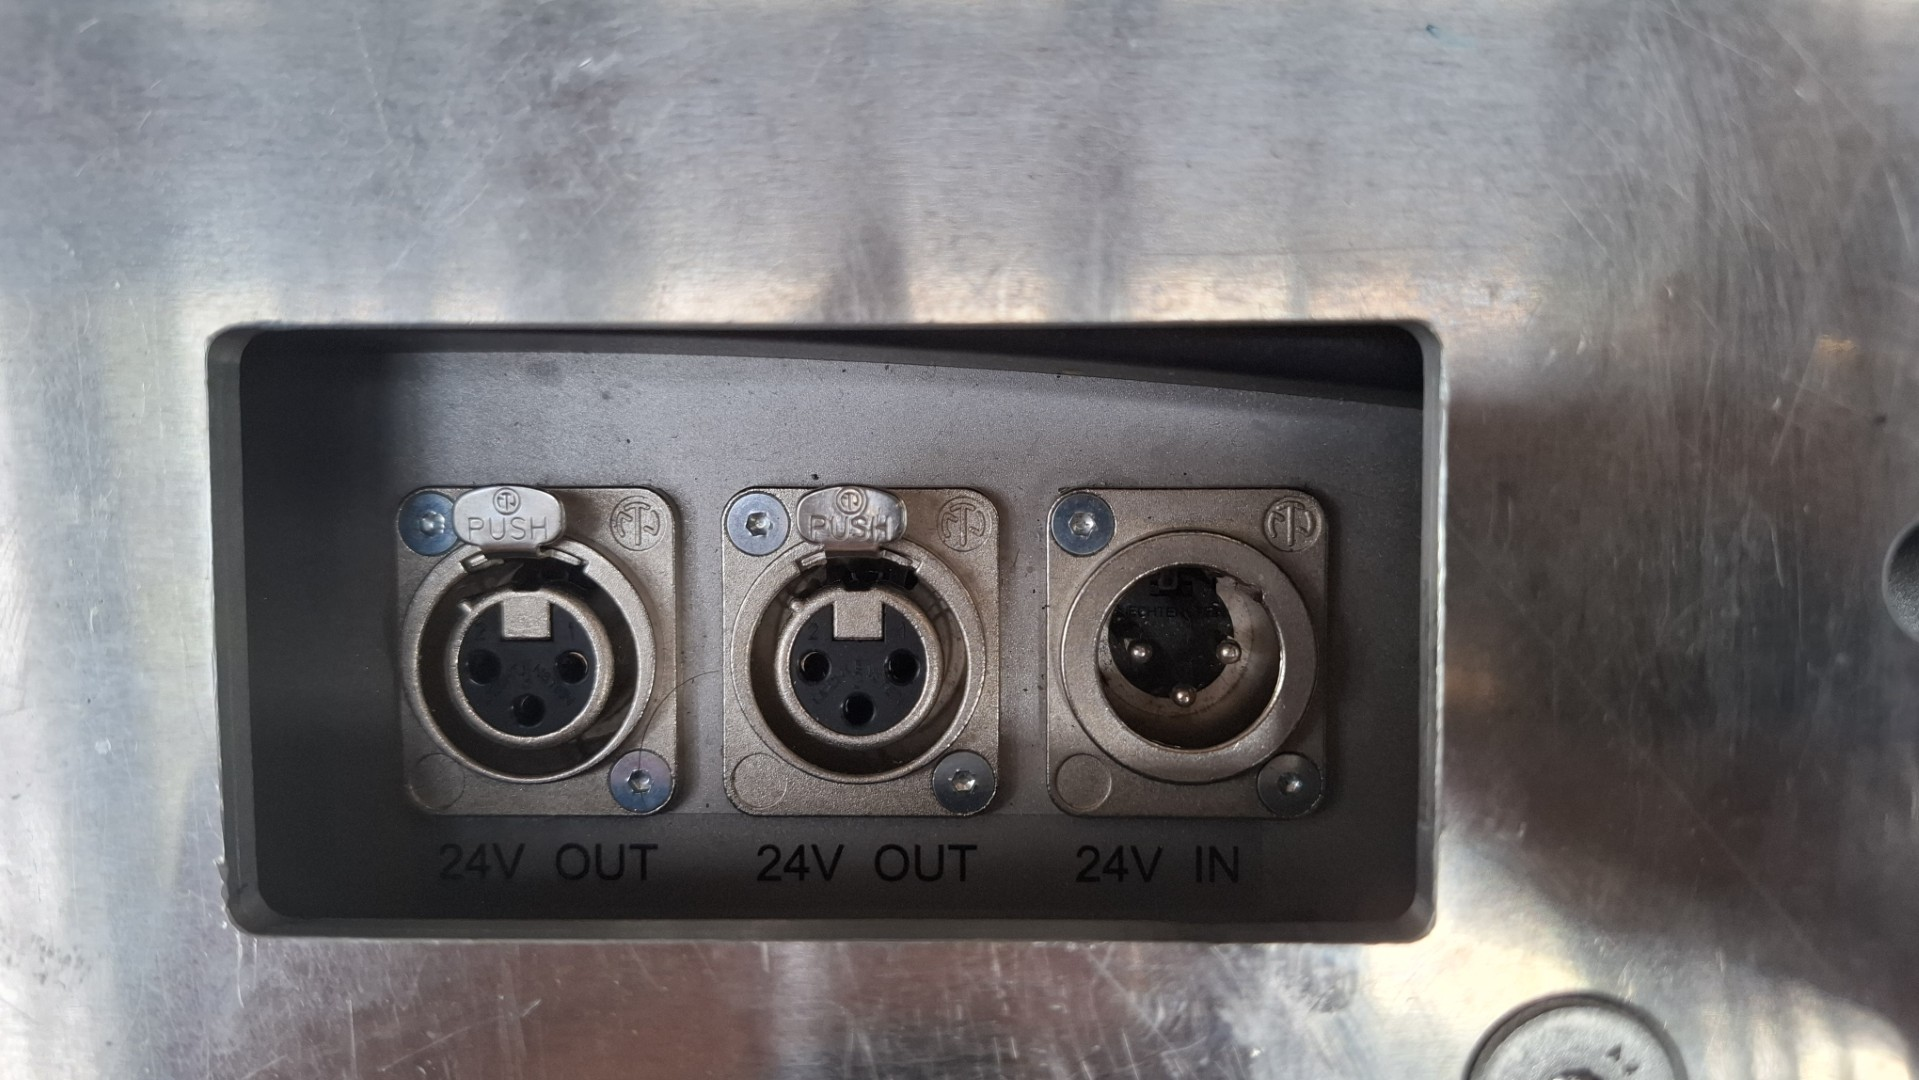
\includegraphics[width=\linewidth]{images/sec2/youbot_power.jpg}
            \caption{The power input and output ports.}
            \label{fig:youbot-power}
        \end{subfigure}
        \hfill
        \begin{subfigure}[t]{0.49\linewidth}
            \centering
            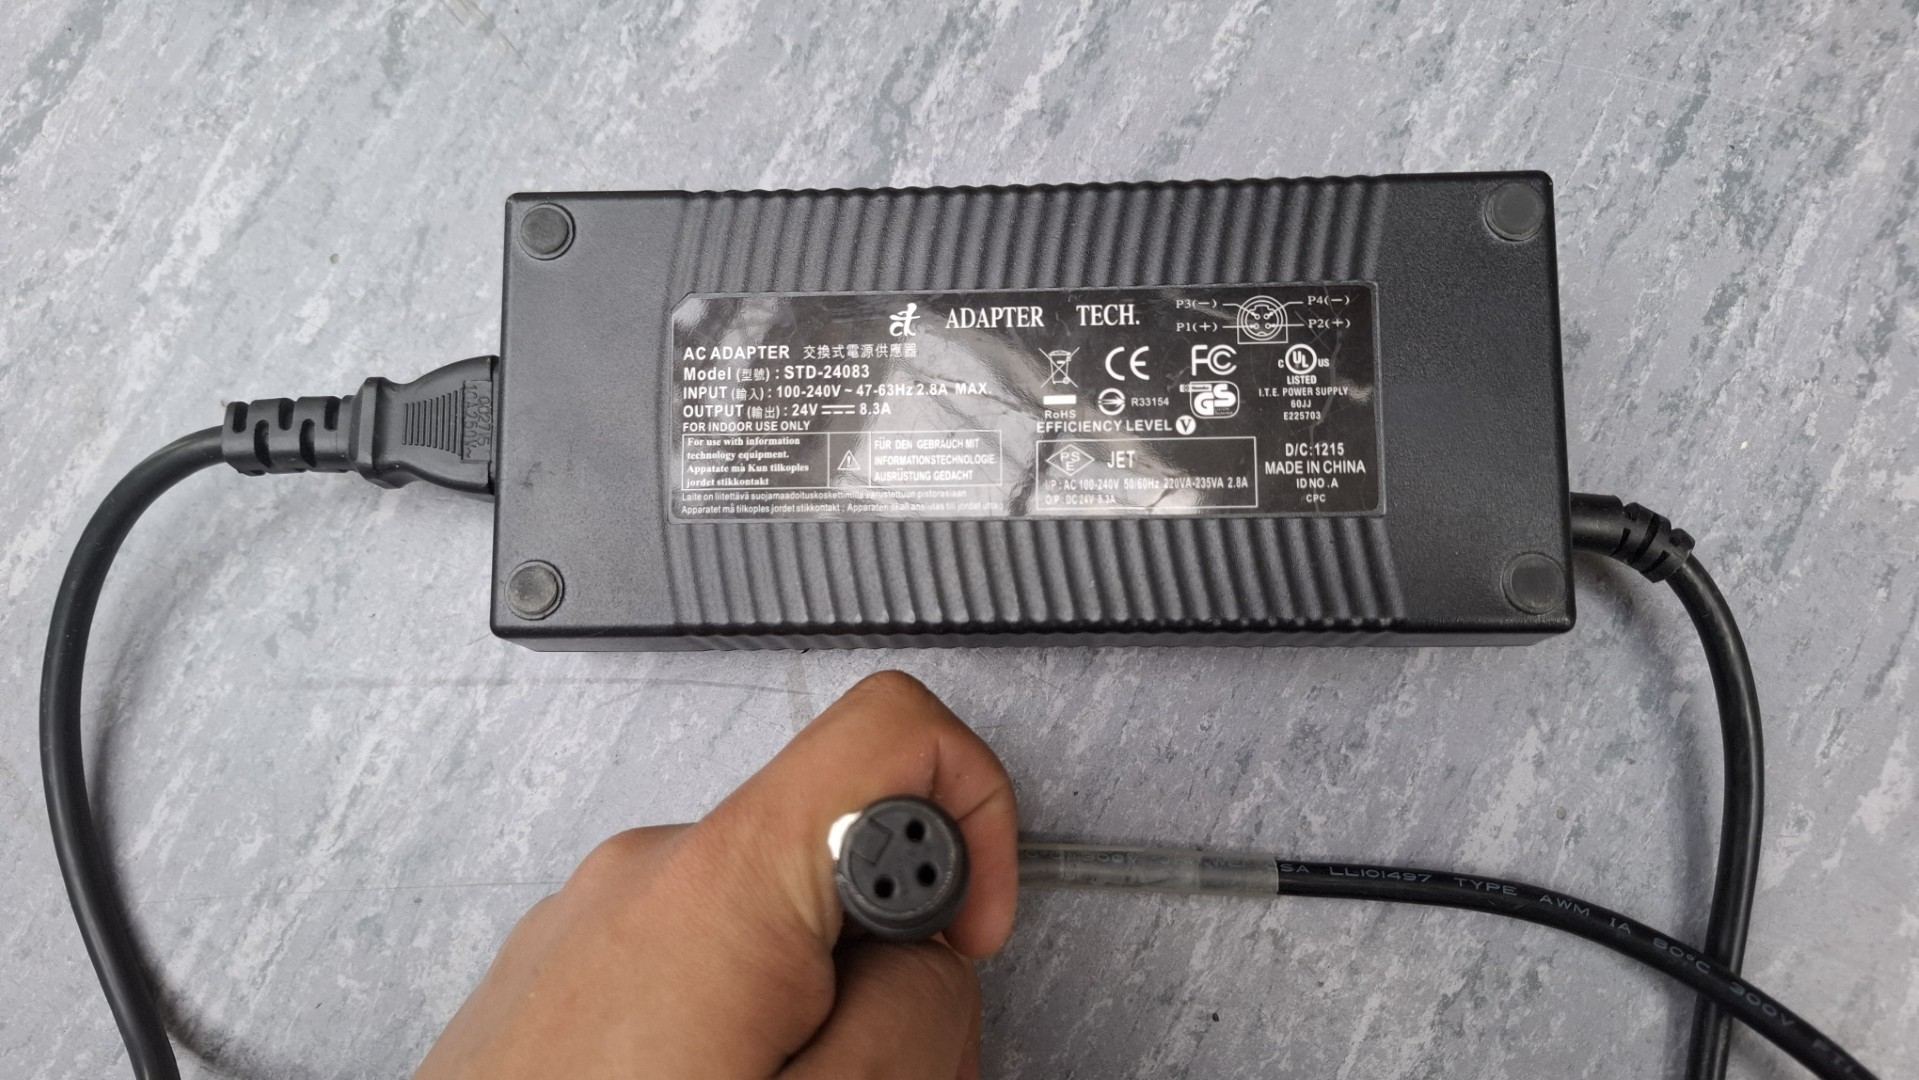
\includegraphics[width=\linewidth]{images/sec2/power_adapter.jpg}
            \caption{The 24V power adapter used to power the YouBot.}
        \end{subfigure}
        \caption{Direct power supply components for the YouBot.}
    \end{figure}

    However, continuously powering the YouBot through a wall connection is not ideal for the goal of mobile robotics. Thus, the YouBot was also originally equipped with a maintainence-free sealed lead-acid (SLA) battery (Figure~\ref{fig:youbot-battery}) . This battery had a capacity of 5Ah and provided an approximate runtime of 90 minutes \cite{YouBotSpecs2016}. This battery furthermore connects to the robot via a 4-pin XLR connector, and is located in a dedicated slot on the left side of the robot (Figure~\ref{fig:youbot-battery-holder}). %While the 4-pin XLR connector is not standard for power supply (it is typically used for audio equipment), it is very robust and secure for the purposes of a mobile robot. This lead-acid battery is of dimensions 23cmx9.4cmx7.3cm.

    \begin{figure}[H]
        \centering
        \begin{subfigure}[t]{0.49\linewidth}
            \centering
            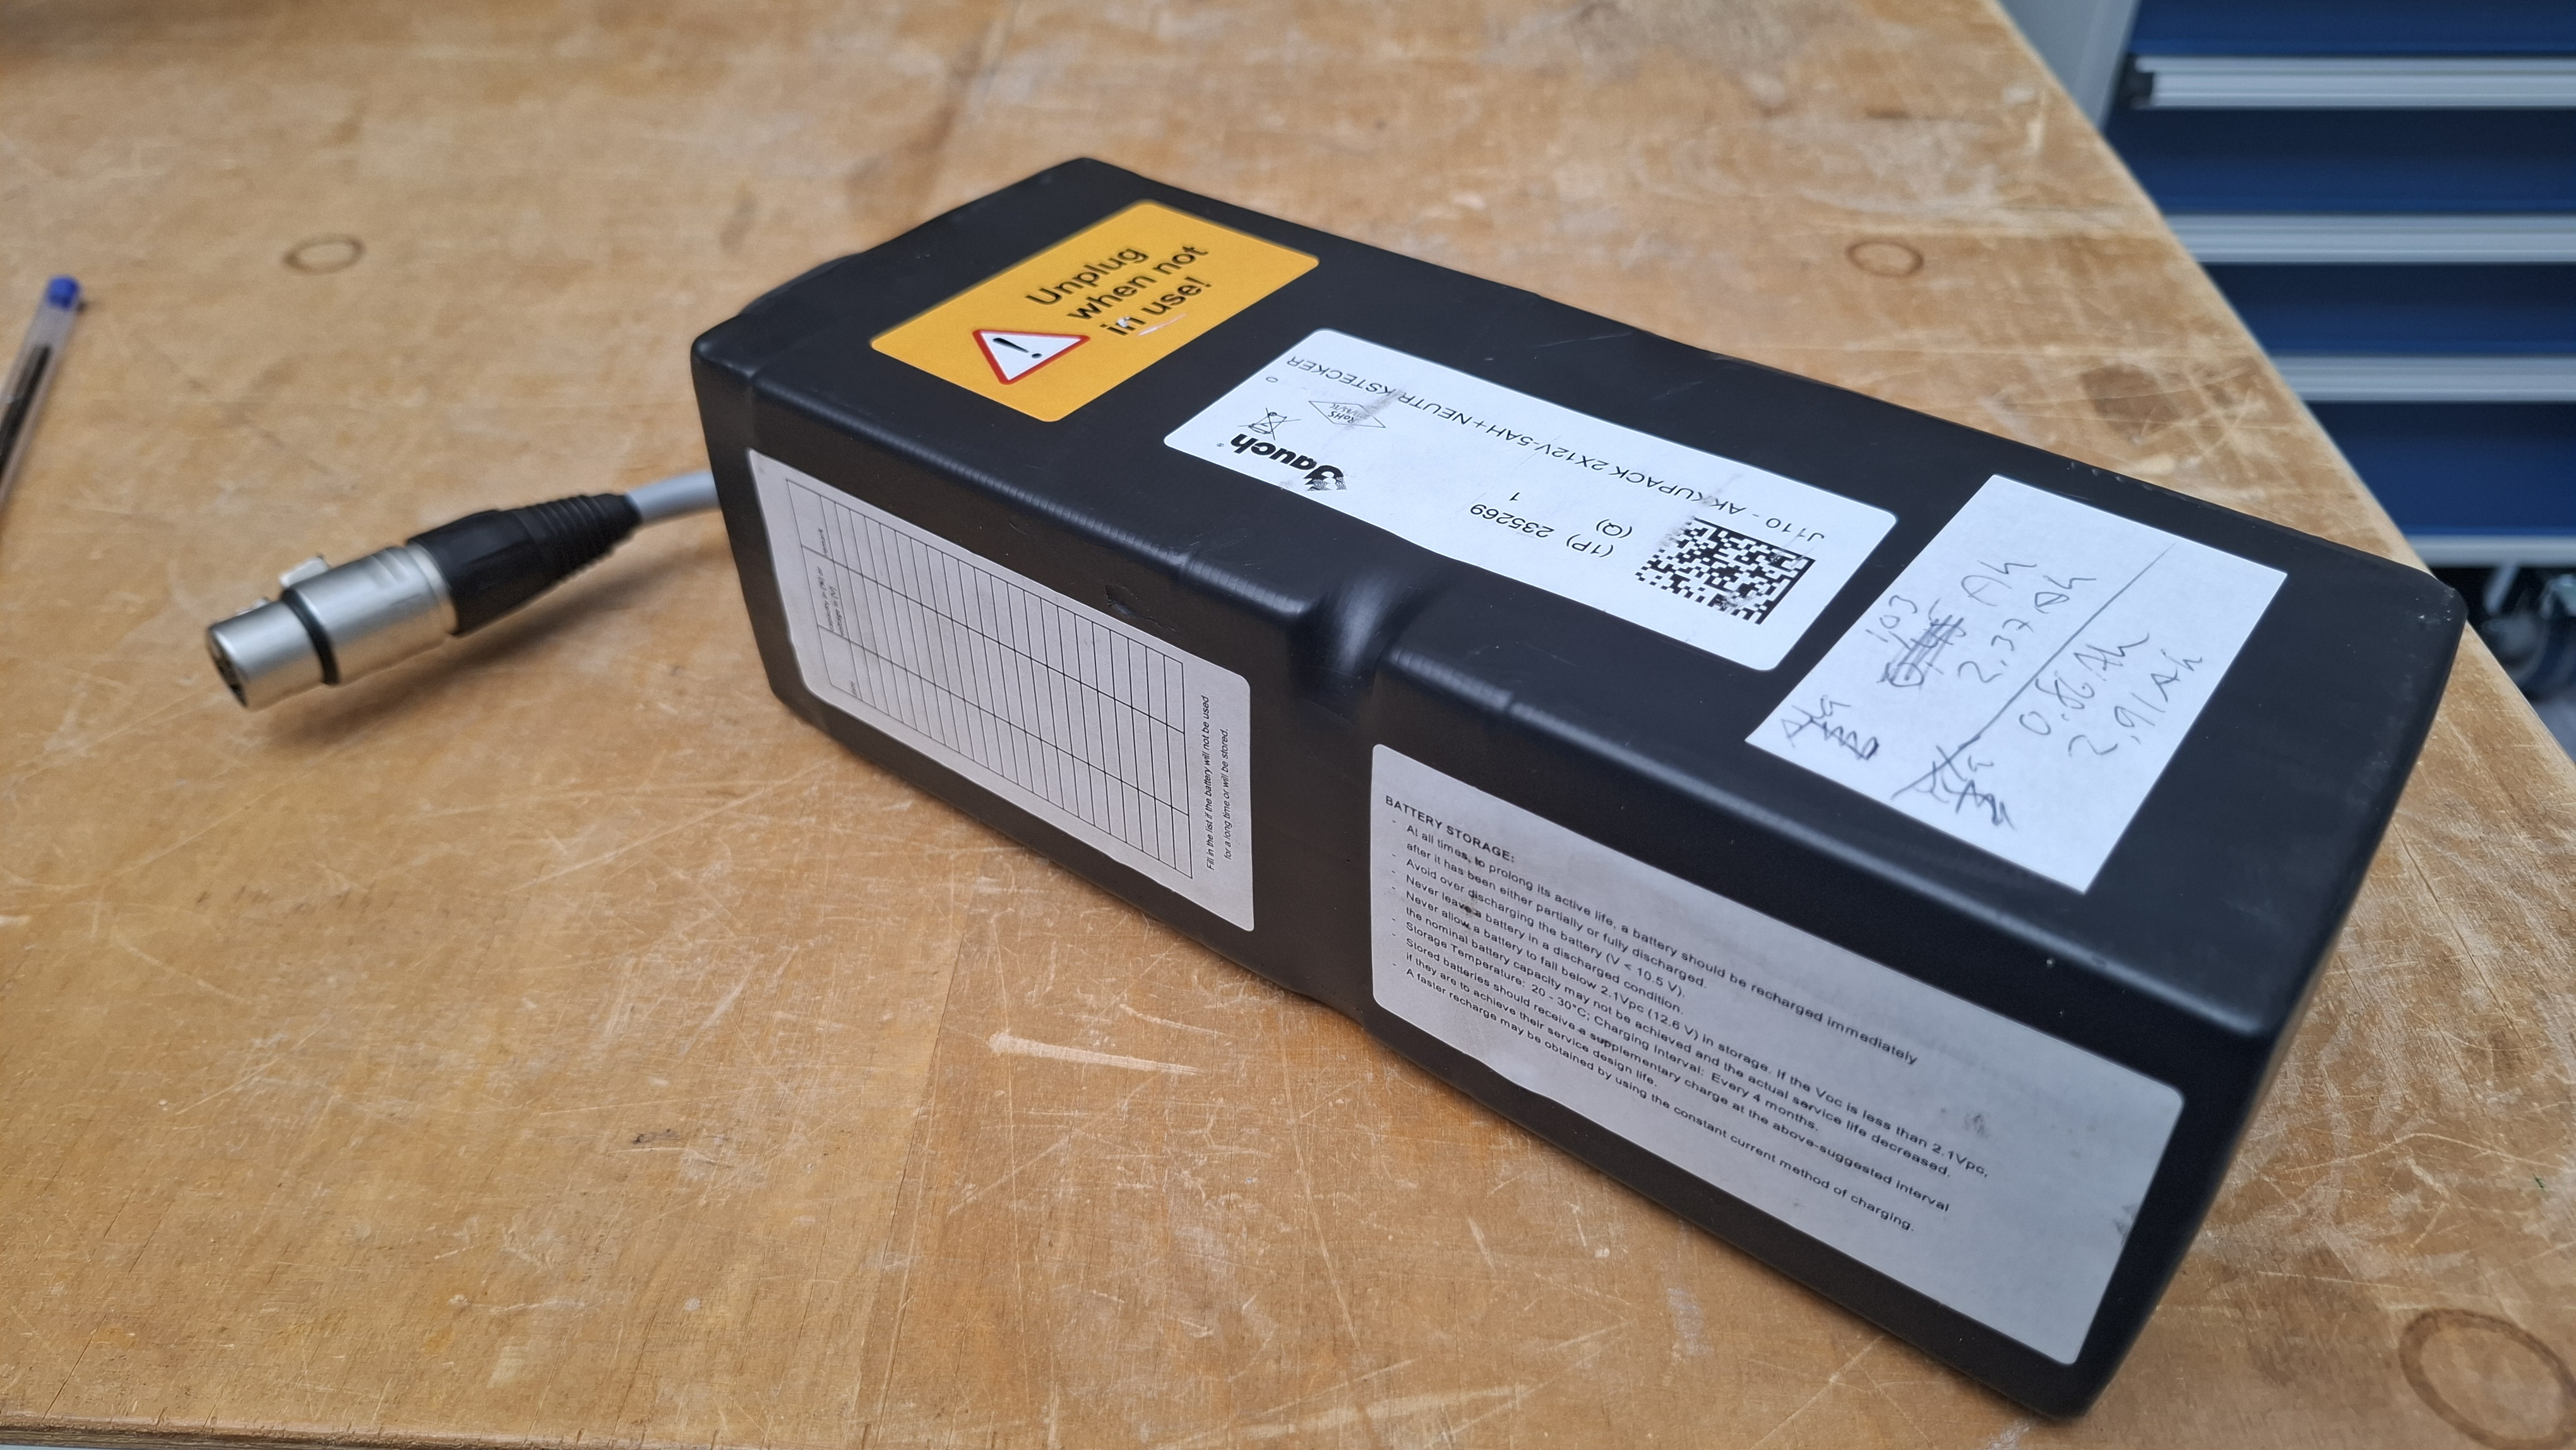
\includegraphics[width=\linewidth]{images/sec2/youbot_battery.jpg}
            \caption{The original SLA battery.}
            \label{fig:youbot-battery}
        \end{subfigure}
        \hfill
        \begin{subfigure}[t]{0.49\linewidth}
            \centering
            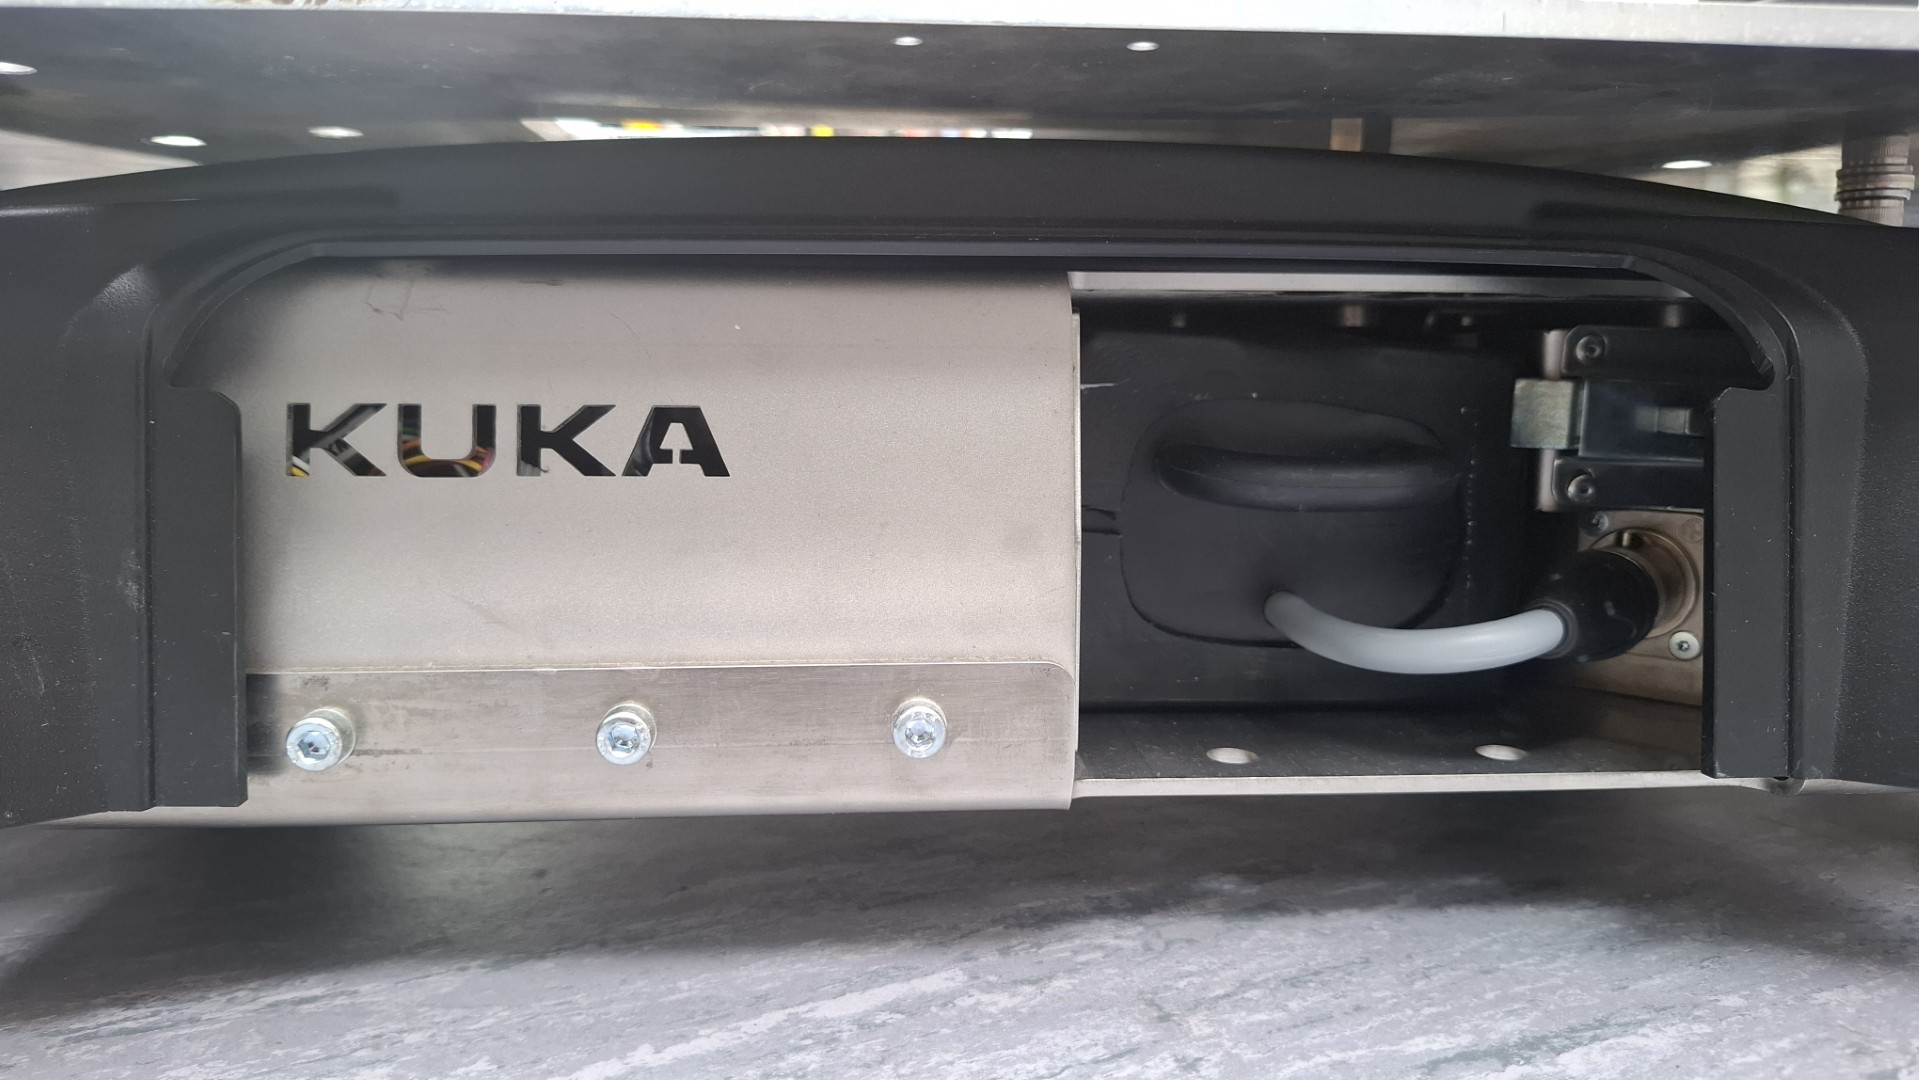
\includegraphics[width=\linewidth]{images/sec2/youbot_battery_holder.jpg}
            \caption{The left side of the robot, showing the battery in its holder.}
            \label{fig:youbot-battery-holder}
        \end{subfigure}
        \caption{The YouBot's SLA Battery.}
    \end{figure}

    Upon receiving the robot, four SLA batteries were available: three of them were the original units supplied with the YouBot, and the fourth was a makeshift replacement assembled by the lab engineer, Vesa Korhonen, in 2019. Unfortunately, none of these batteries were functional. The original units had degraded beyond usability, and the makeshift battery had similarly deteriorated over time.

    As a result, the robot could not operate on battery power in its current state and required a constant wired connection to a wall outlet—an obvious limitation for a mobile robotics platform. A battery replacement would be ideal to restore the robot's potential mobility. 

    \subsection{Sensors}
    
    Alongside the robot base and various hardware components, the YouBot was also equipped with a variety of sensors to enhance perception and navigation. These included a Kinect v1 camera and two Hokuyo URG-04LX laser rangefinders. 

    \subsubsection{Kinect}  

    The Kinect v1 camera is a depth and RGB camera that was originally designed and sold in tandem with the XBOX 360 to support motion tracking and gaming. Due to its low cost, high availability and ease of use, it had indirectly become a popular choice in the robotics community for perception tasks in the 2010s. 

    Access to the Kinect's sensor data can be achieved through the use of open-source software such as libfreenect \cite{OpenKinectLibfreenect}. The retrieved data can then be processed using computer vision libraries such as OpenCV to enable the autonomous navigation as previously described. 

    \begin{figure}[ht]
        \centering
        %/flushleft
        %/flushright
        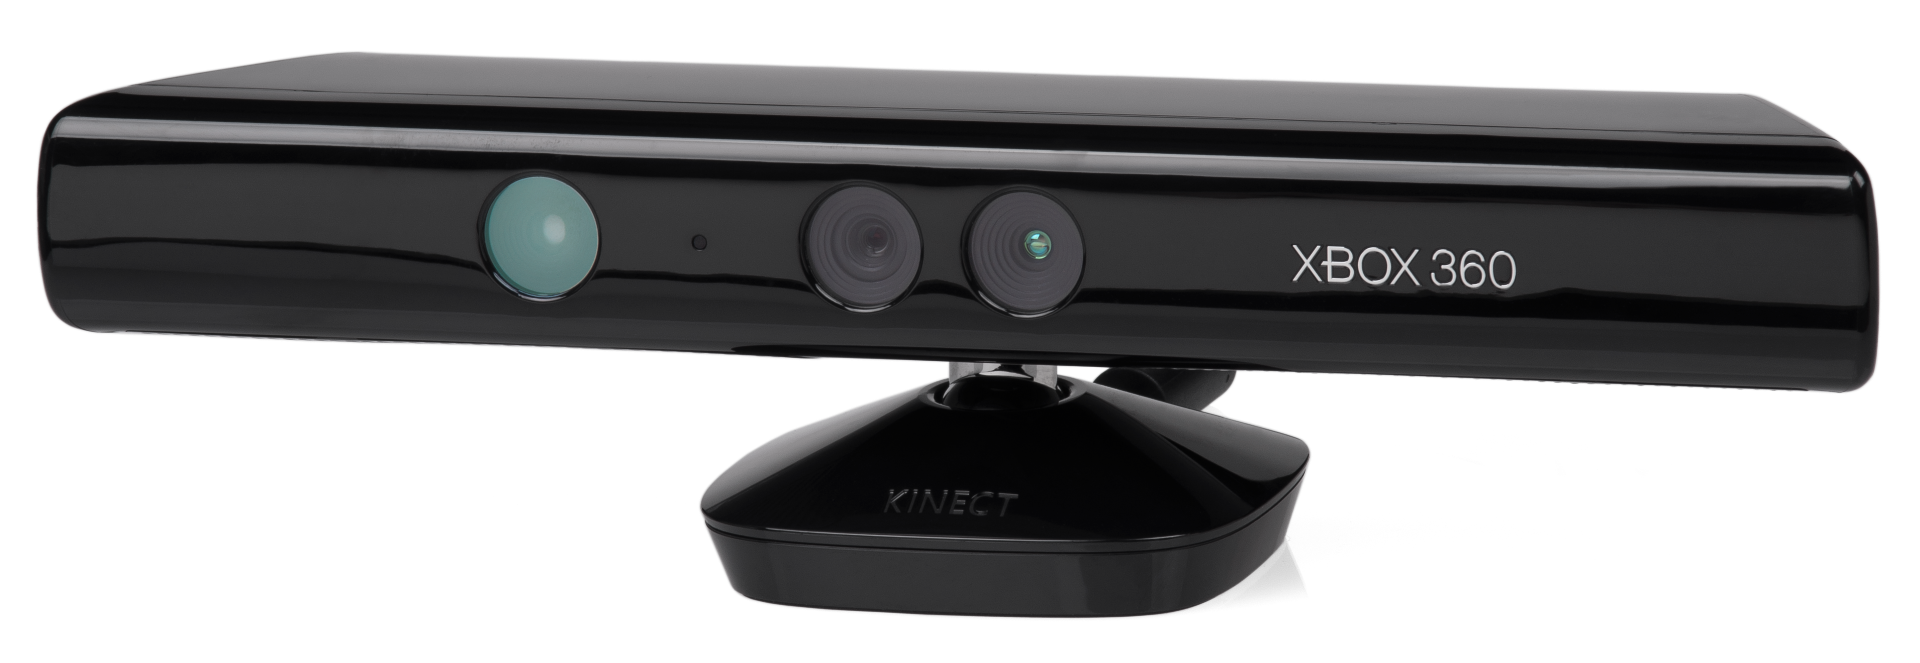
\includegraphics[width=0.5\linewidth]{images/sec2/kinectv1.png}
        \caption{The Kinect v1 camera module.}
    \end{figure}


    \subsubsection{Hokuyo URG-04LX Laser Rangefinder}

    The Hokuyo URG-04LX is a lightweight 2D laser rangefinder that is commonly used in robotics research. It provides distance measurements in a 240-degree field of view and can detect objects upto 5.6m meters away with an accuracy of \(\pm30\) mm and angular resolution of 0.352deg \cite{HokuyoURG04LXUG01}. It communicates with the onboard computer using a serial interface, enabling straightforward integration into existing systems for mapping, localization, and obstacle avoidance tasks. 

    \begin{figure}[ht]
        \centering
        %/flushleft
        %/flushright
        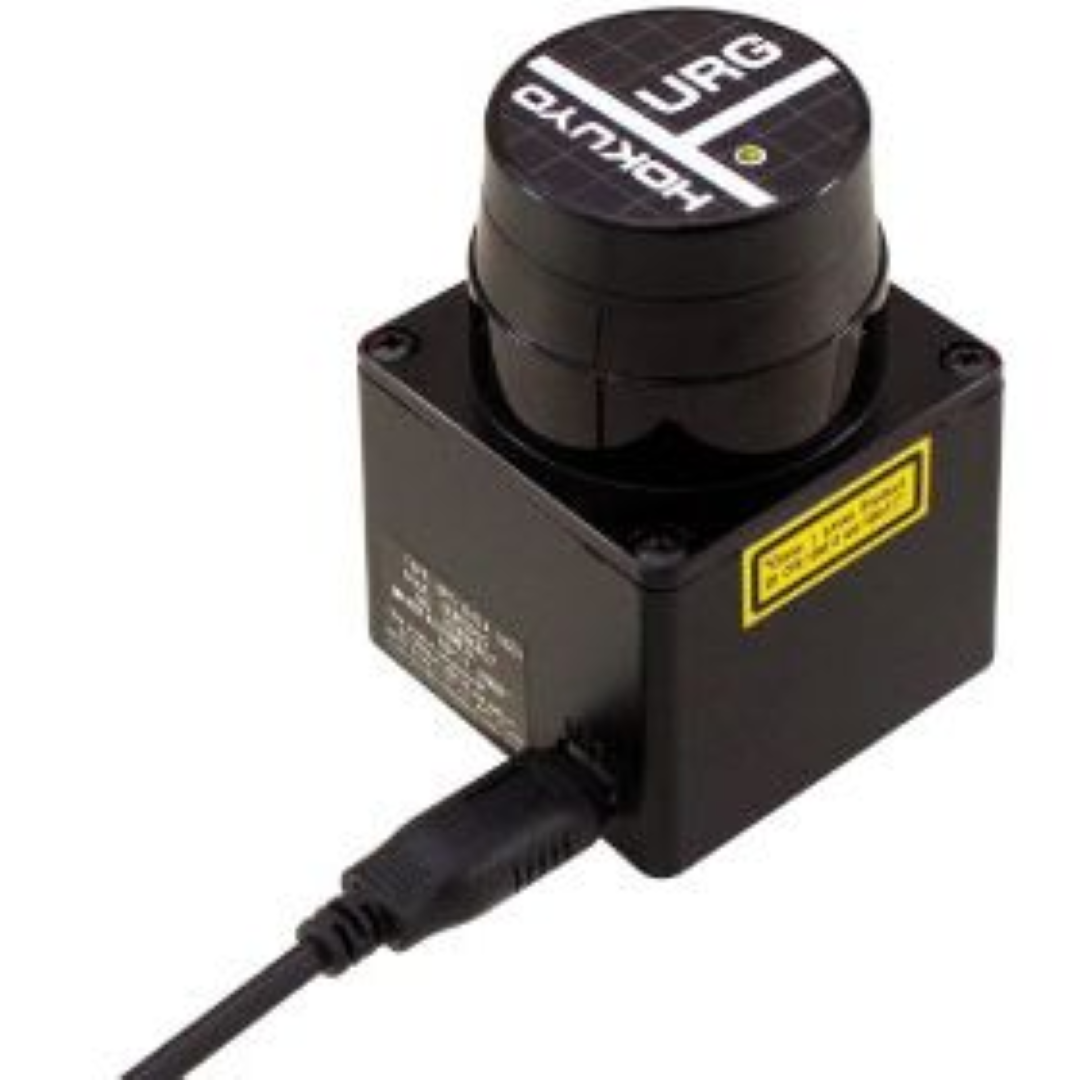
\includegraphics[width=0.25\linewidth]{images/sec2/hokuyo.png}
        \caption{The Hokuyo URG-04LX laser rangefinder.}
    \end{figure}

    \subsection{Additional Hardware Components}

    The YouBot also came with a variety of additional components and accessories to assist with sensor mounting and operation. These included a variety of nuts, bolts, and screws, as well as a hex key and several horizonal and vertical pillars. These components can be combined in a variety of ways to create a stable and secure mounting platform for the sensors. 

    A key component provided was a pre-attached sensor and mounting plate on the top panel (see Figure~\ref{fig:youbot-aalto}), designed to also assist in the convenient attachment of various sensors and accessories \cite{YouBotSensorPlate2016}. A wireless adapter was also included, which can be used to connect to the internet without the need of Ethernet. Additionally, a separate box contained various miscellaneous items, including previously used batteries, panels for the Youbot and controllers; which could prove potentially useful for customization or repair. 

    
    \begin{figure}[H]
        \centering
        \begin{subfigure}[t]{0.49\linewidth}
            \centering
            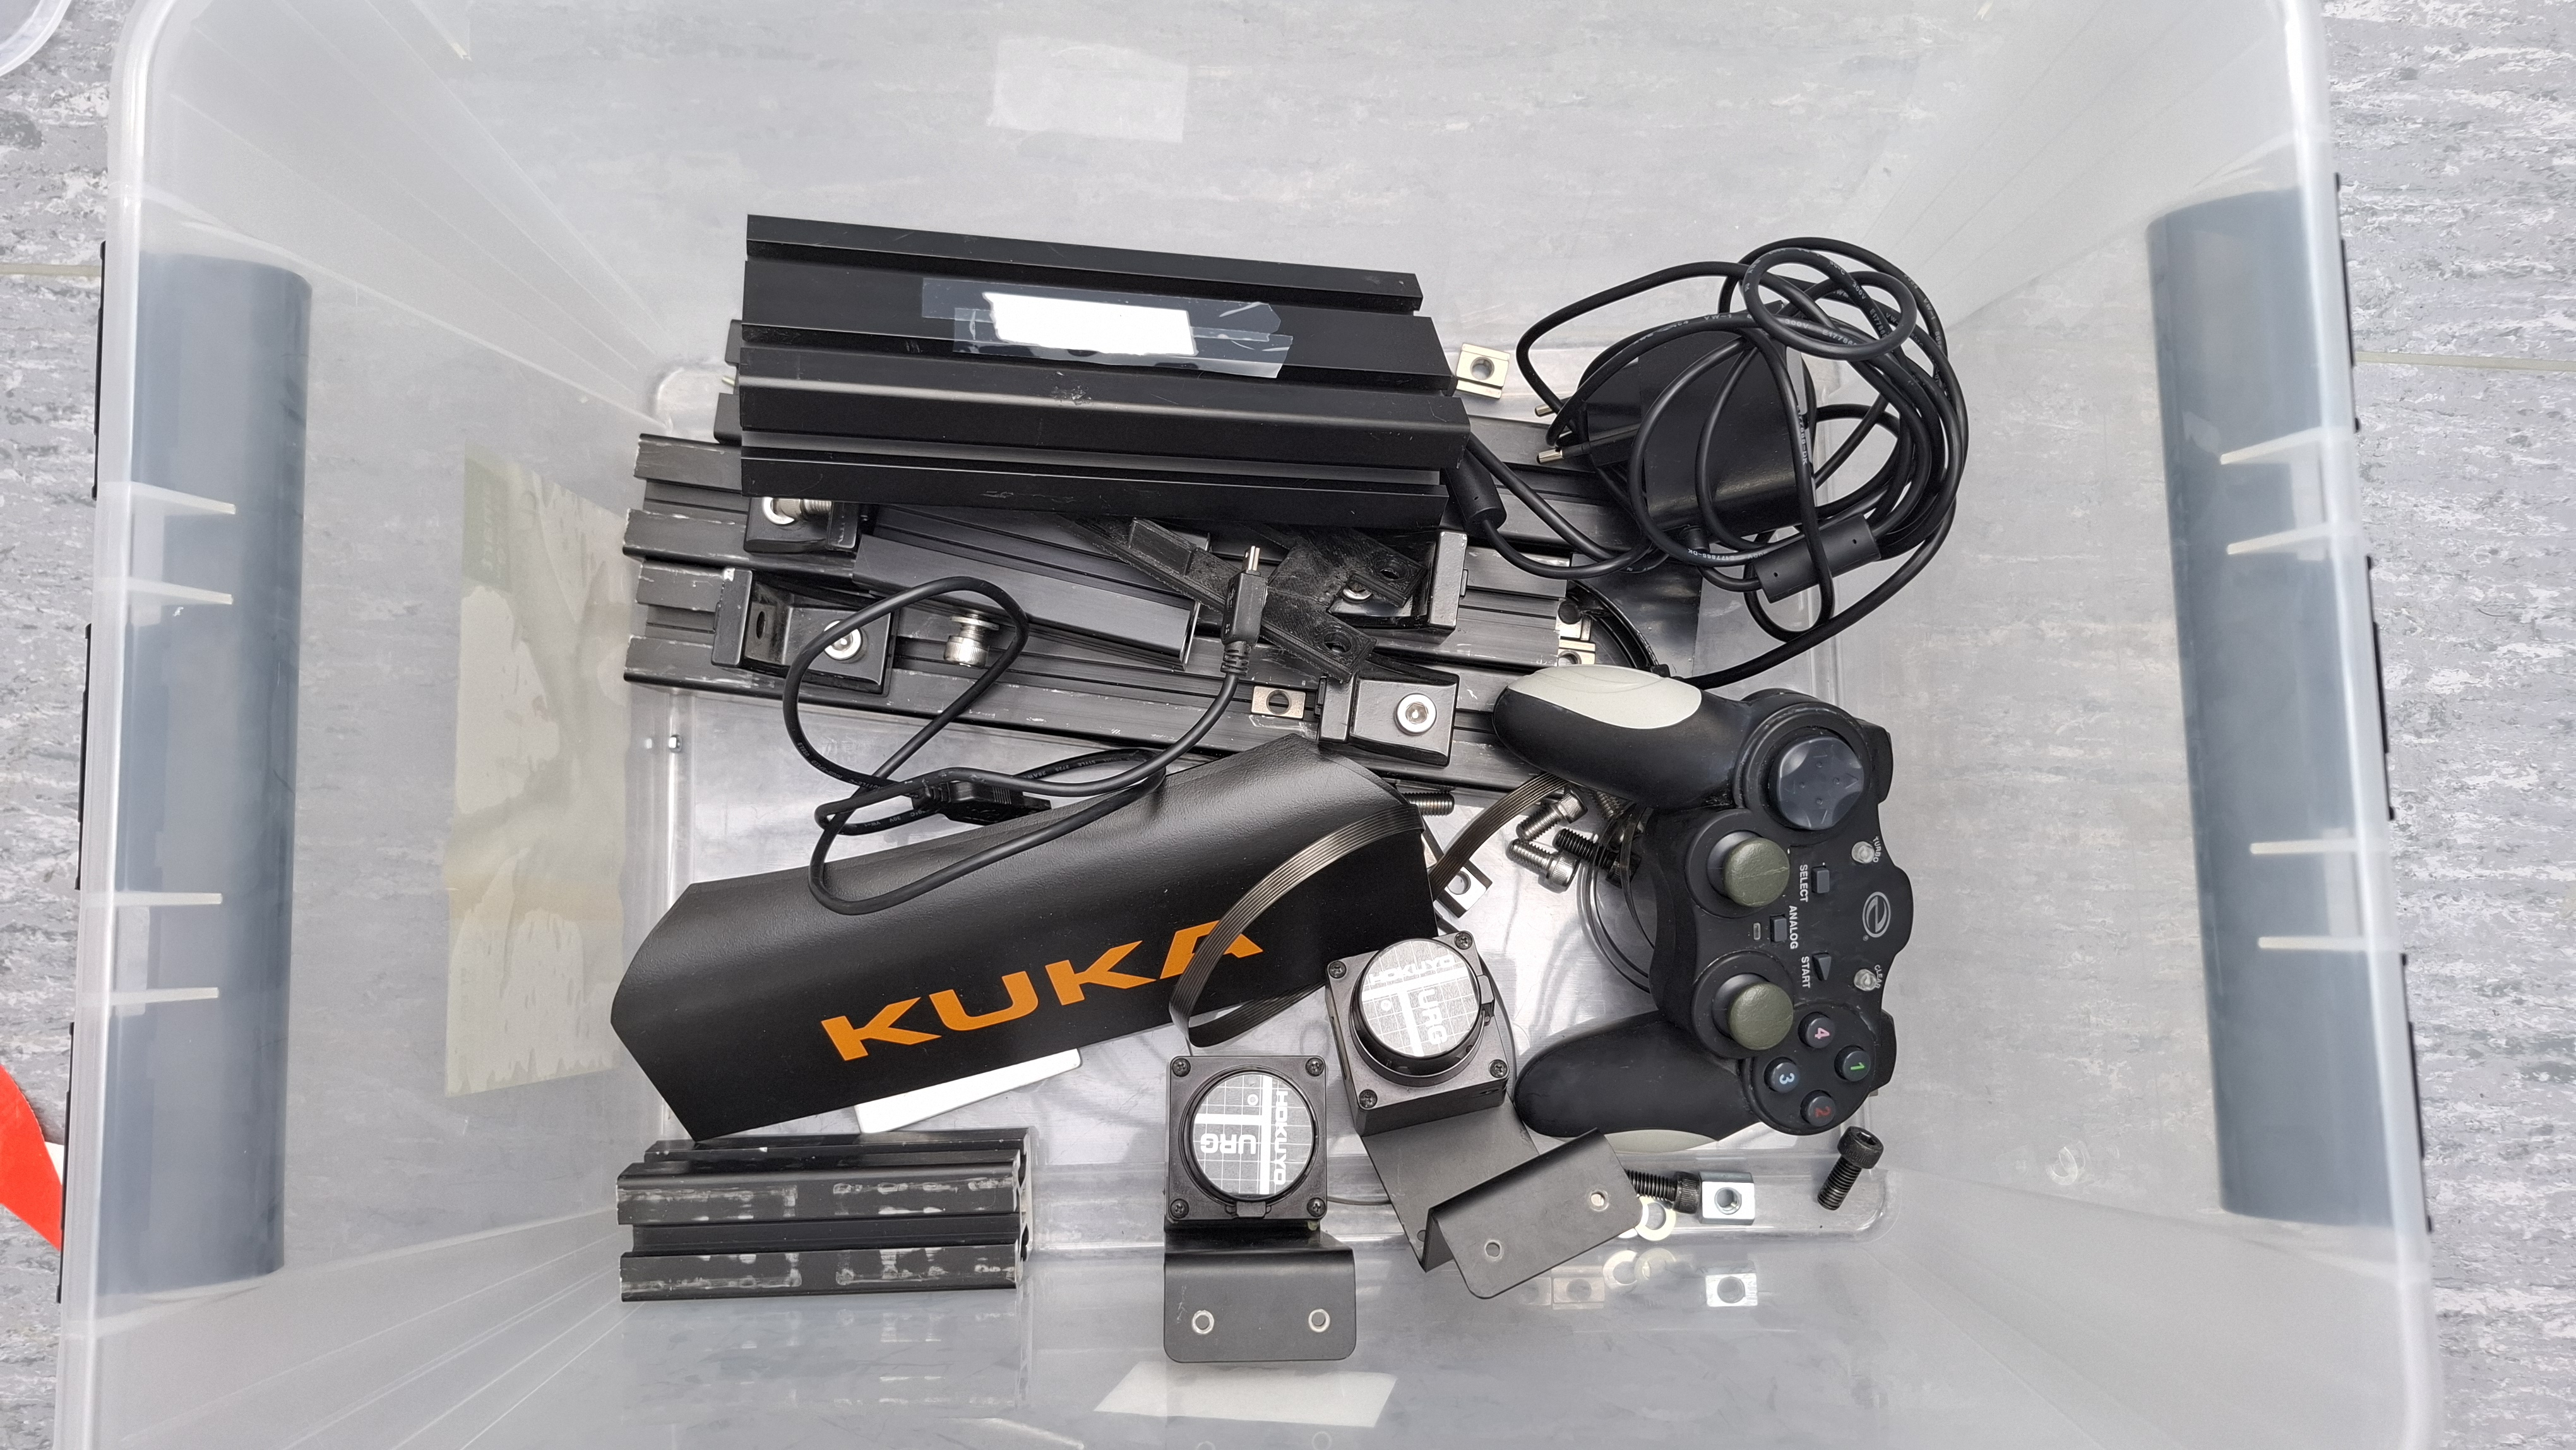
\includegraphics[width=\linewidth]{images/sec2/box2.jpg}
            \caption{Various pillars, nuts and bolts amongst other components.}
        \end{subfigure}
        \hfill
        \begin{subfigure}[t]{0.49\linewidth}
            \centering
            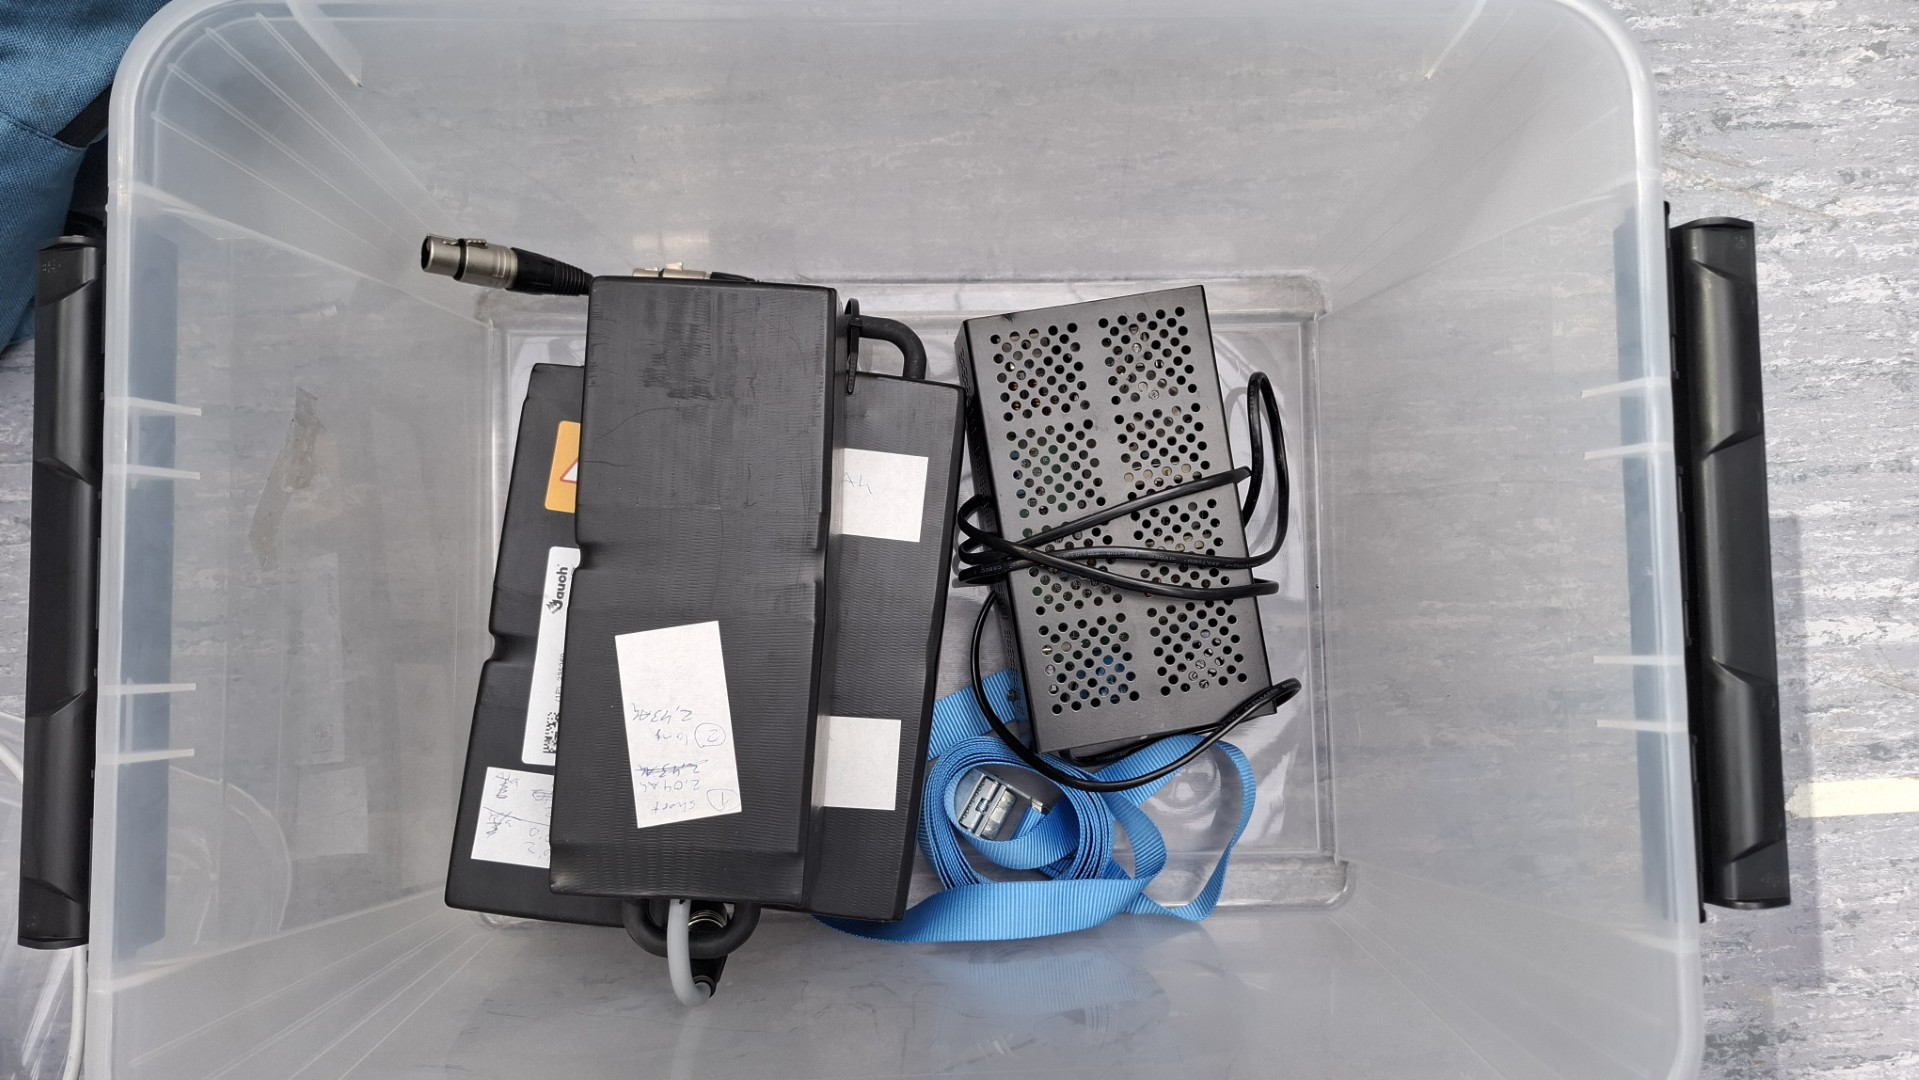
\includegraphics[width=\linewidth]{images/sec2/box1.jpg}
            \caption{The box containing previously used batteries and miscellaneous components.}
        \end{subfigure}

        \caption{Additional hardware components supplemented with the YouBot.}
    \end{figure}

    \subsection{Documentation}
    
    The documentation for the KUKA YouBot is sparse. Since the product's discontinuation in the mid-2010s, KUKA has removed most references to the product from their official website, and the official website for the YouBot (\texttt{youbot-store.com}) is no longer active. The only starting point for official documentation was through a user manual dated 2013 found on the onboard PC \cite{KUKAYouBotManual2013}.

    Fortunately, as the YouBot was marketed as an open-source platform, many of its drivers and software components remain available on the YouBot GitHub repositories \cite{githubYoubotOverview}. Furthermore, we leveraged the Internet Archive's Wayback Machine \cite{WaybackMachine} to retrieve snapshots of the original website. While this archive is incomplete and tedious to comb through, they provide valuable insights into the hardware specifications, software stack, and applications of the YouBot during its active develpoment period. Furthermore, the youbot official GitHub repository \cite{githubYoubotOverview} contains all original packages and software components. Driver documentation is additionally available on a dedicated GitHub page \cite{janpaulusYouBotDriver}.

    \begin{figure}[ht]
        \centering
        \begin{subfigure}[t]{0.49\linewidth}
            \centering
            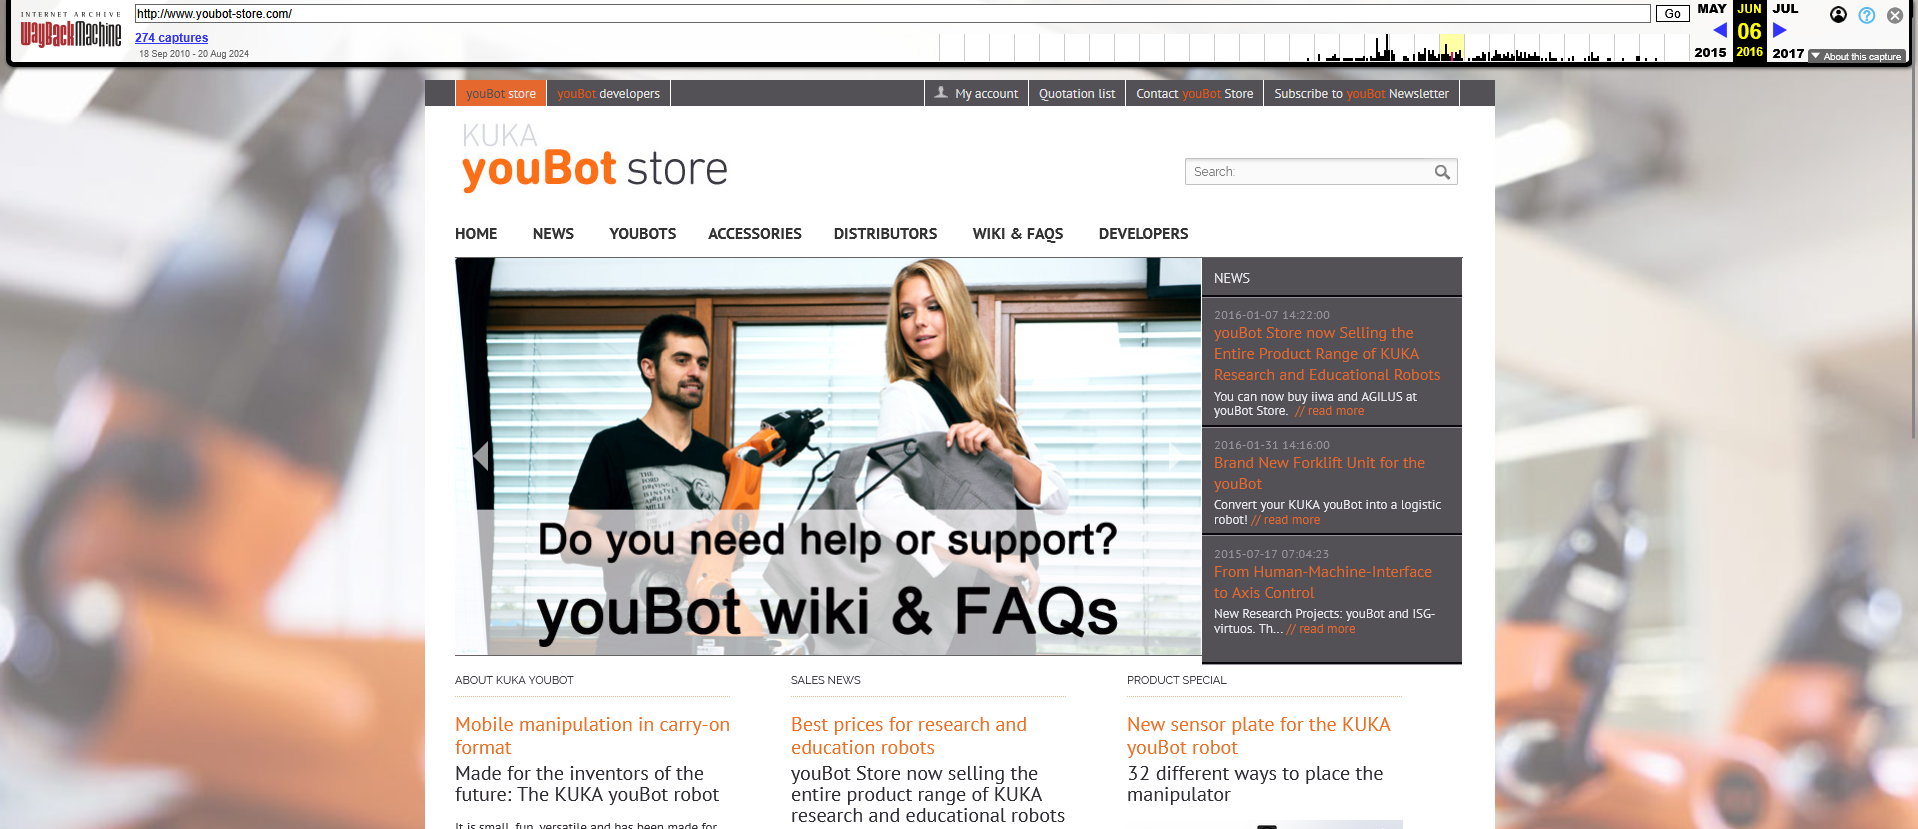
\includegraphics[width=\linewidth]{images/sec2/youbot-store-page.png}
            \caption{The YouBot Store page on the Internet Archive's Wayback Machine.}
        \end{subfigure}
        \hfill
        \begin{subfigure}[t]{0.49\linewidth}
            \centering
            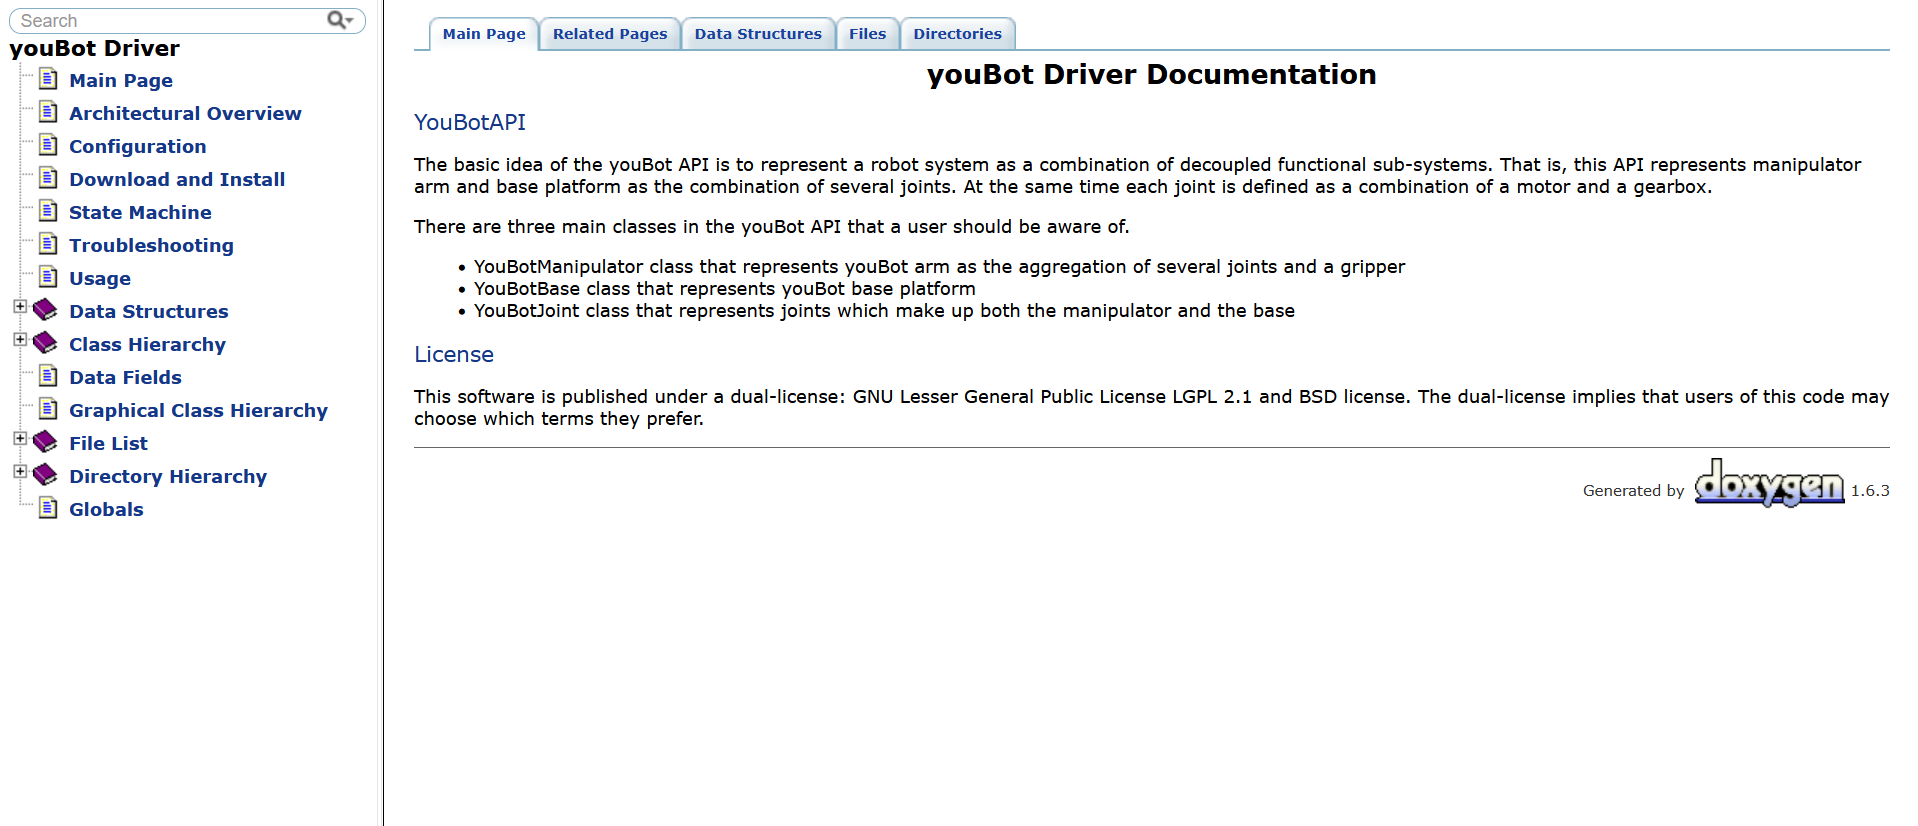
\includegraphics[width=\linewidth]{images/sec2/janpalaus.png}
            \caption{The YouBot driver documentation on GitHub Pages.}
        \end{subfigure}
        \caption{Websites for YouBot documentation.}
\end{figure}
   

    \subsection{Initial Project Goals}

    Considering the hardware and software components of the YouBot, the initial goals of this project involved a comprehensive revival of the robot and the enabling of autonomous navigation using the Kinect camera. This would showcase the potential of the YouBot in cutting-edge research despite its age. 

    The Teach \& Repeat (T\&R) method \cite{Shahrivar2018} was considered to be an ideal candidate to allow for autonomous navigation. This is a two-phase robotic navigation method where a robot is first "taught" a path via human guidance or pre-recoded data. The sensor data captured during this phase can then be used to allow the robot to autonomously "repeat" the path later on, even in different environments.

    T\&R only requires a single camera for a basic implementation. It is a relatively simple method to implement through the use of open-source software and libraries, such as OpenCV and ROS. Furthermore, it is robust to changes in the environment and can dynamically correct errors through the use of visual odometry. As such, it has been a very popular research topic within the field of robotics, particularly in the context of mobile robots \cite{10611662,NITSCHE2020103577}. Much of the work done on extending T\&R aims to improve this robustness and scalability for a variety of sensors and use-cases. 

    \begin{figure}[ht]
        \centering
        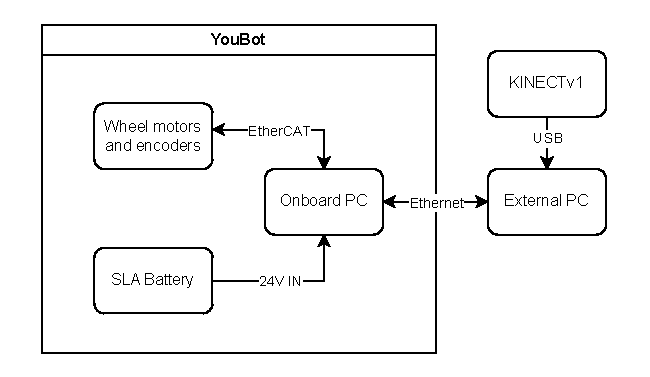
\includegraphics[width=0.8\linewidth]{diagrams/sample.pdf}
        \caption{System Diagram}
        \label{fig:system-diagram}
    \end{figure}

    Figure~\ref{fig:system-diagram} shows the proposed system architecture for this implementation. This would involve the onboard PC running ROS 1 Hydro, which would handle the low-level control tasks regarding motor actuation. The navigation and perception tasks would be handled by a more capable external computer running ROS 2 Jazzy. The two systems would then communicate through a ROS1-ROS2 bridge,  enabling compatibility between legacy software on the YouBot and the more modern ROS2 stack. The Kinect camera would be then mounted on top of the YouBot, and would be connected to the external computer via USB. This setup allows for the YouBot to be used without much modification or strain to its legacy hardware, while still enabling the use of modern software and sensors.

    However, due to several challenges—namely the age of the YouBot, limited prior experience with robotics, and software incompatibilities—this plan proved infeasible. A revised set of project goals was subsequently developed, as discussed in the following section.

    \pagebreak
    
    \section{Project Overview}

    \subsection{Technical Goals}

    The technical goals for this project involve the deployment and quantification of the robot's capabilities, particularly in terms of navigation and odometry. This would involve the following goals: 
    \begin{itemize}[noitemsep, topsep=0pt]
        \item Inspecting the initial physical state of the YouBot
        \item Enabling the robot start up
        \item Enabling the running of the original demos
        \item Enabling the running of the ROS interface
        \item Enabling the ROS1-ROS2 bridge
        \item Enabling wireless connections to external computers using SSH and Ethernet
        \item Writing custom programs to control the YouBot
        \item Testing the movement and odometry of the YouBot
        \item Measuring the quality of movement and odometry by measuring their error
        \item Replacing the current deprecated batteries with a usable battery
        \item Documenting the revival process and potential future applications of the YouBot
    \end{itemize}
    
    The set of goals that have been formulated have deviated from the original goals, which were formulated based on experimenting and identifying the limitations of the robot. 

    \subsection{Learning Objectives}

    In parallel with technical outcomes, this project required gaining a range of practical and theoretical competencies in robotics. These learning objectives included:
    \begin{itemize}[noitemsep, topsep=0pt]
        \item Gaining hands-on experience restoring and operating a legacy robotic platform (KUKA YouBot)
        \item Building proficiency in Linux environments relevant to robotics development
        \item Writing Bash scripts to automate system setup, compilation, and deployment workflows
        \item Understanding the architecture and functionality of both ROS1 and ROS2, including their integration
        \item Establishing and managing secure connections between host and robot using SSH and Ethernet
        \item Creating and deploying custom ROS nodes for low-level motion control
        \item Studying robot navigation and odometry principles, including error sources and correction strategies
        \item Developing skills for documenting restoration efforts and formulating directions for future work
    \end{itemize}

    \subsection{System Architecture}
    Our current system architecture is starkly different from the initial goal. While the YouBot itself remains unchanged, the external computer only serves the purpose of SSH access and remote control into the onboard computer. SSH could be conveniently done through a wireless connection, or through a more reliable Ethernet connection. The onboard computer runs ROS1 Hydro and communicates with the wheel motors and encoders through EtherCAT. No external sensors will be used, highlighting our focus on enabling the YouBot's existing capabilities rather than extending them. 
    
    \begin{figure}[H]
        \centering
        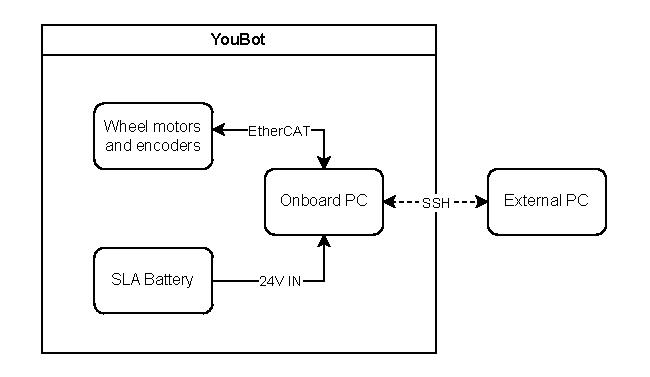
\includegraphics[width=\linewidth]{diagrams/new_arch.drawio.pdf}
        \caption{New System Diagram}
        \label{fig:new-system-diagram}
    \end{figure}

    \pagebreak

    \section{System Development}
    \subsection{Booting up the YouBot}

    After conducting the initial inspection as described in section 2, the next step was to boot up the YouBot. Since the onboard battery was completely dead, the YouBot was connected to an external 24V supply. On long pressing the power button, the screen flashed on and I could see the voltage input for the robot, alongside options to turn the PC and motors on/off seperately.
    
    Using a VGA monitor and USB peripherals, the onboard PC was accessed. It booted successfully and functioned like a standard Linux desktop. The wireless adapter was also operational and could connect to the internet. However, remote access via SSH was initially unavailable due to the absence of a static IP configuration.

    Upon further inspection, several YouBot-specific software packages were also found installed on the onboard computer. These packages include the \code{youbot_driver}, which provides the necessary drivers to communicate with the roboto's motors through EtherCAT, and the \code{youbot_ros_pkg}, which provides a complete ROS stack for the YouBot. These packages are essential for enabling the YouBot to communicate with ROS and to control its motors and sensors. Alternatively, a simpler ROS interface can be used through the \code{youbot_driver_ros_interface} package, which provides a minimal set of ROS nodes to control the YouBot. This package has been used for the purposes of this project to simplify the interaction with the robot. Additionally, the \code{youbot_description} package provides the necessary URDF files to describe the robot's kinematics and dynamics, allowing for simulation and visualization in RViz and Gazebo. Finally, the \code{youbot_applications} package provides a set of example applications and demos to get started with the YouBot.

    \begin{figure}[H]
        \centering
        \begin{subfigure}[t]{0.49\linewidth}
            \centering
            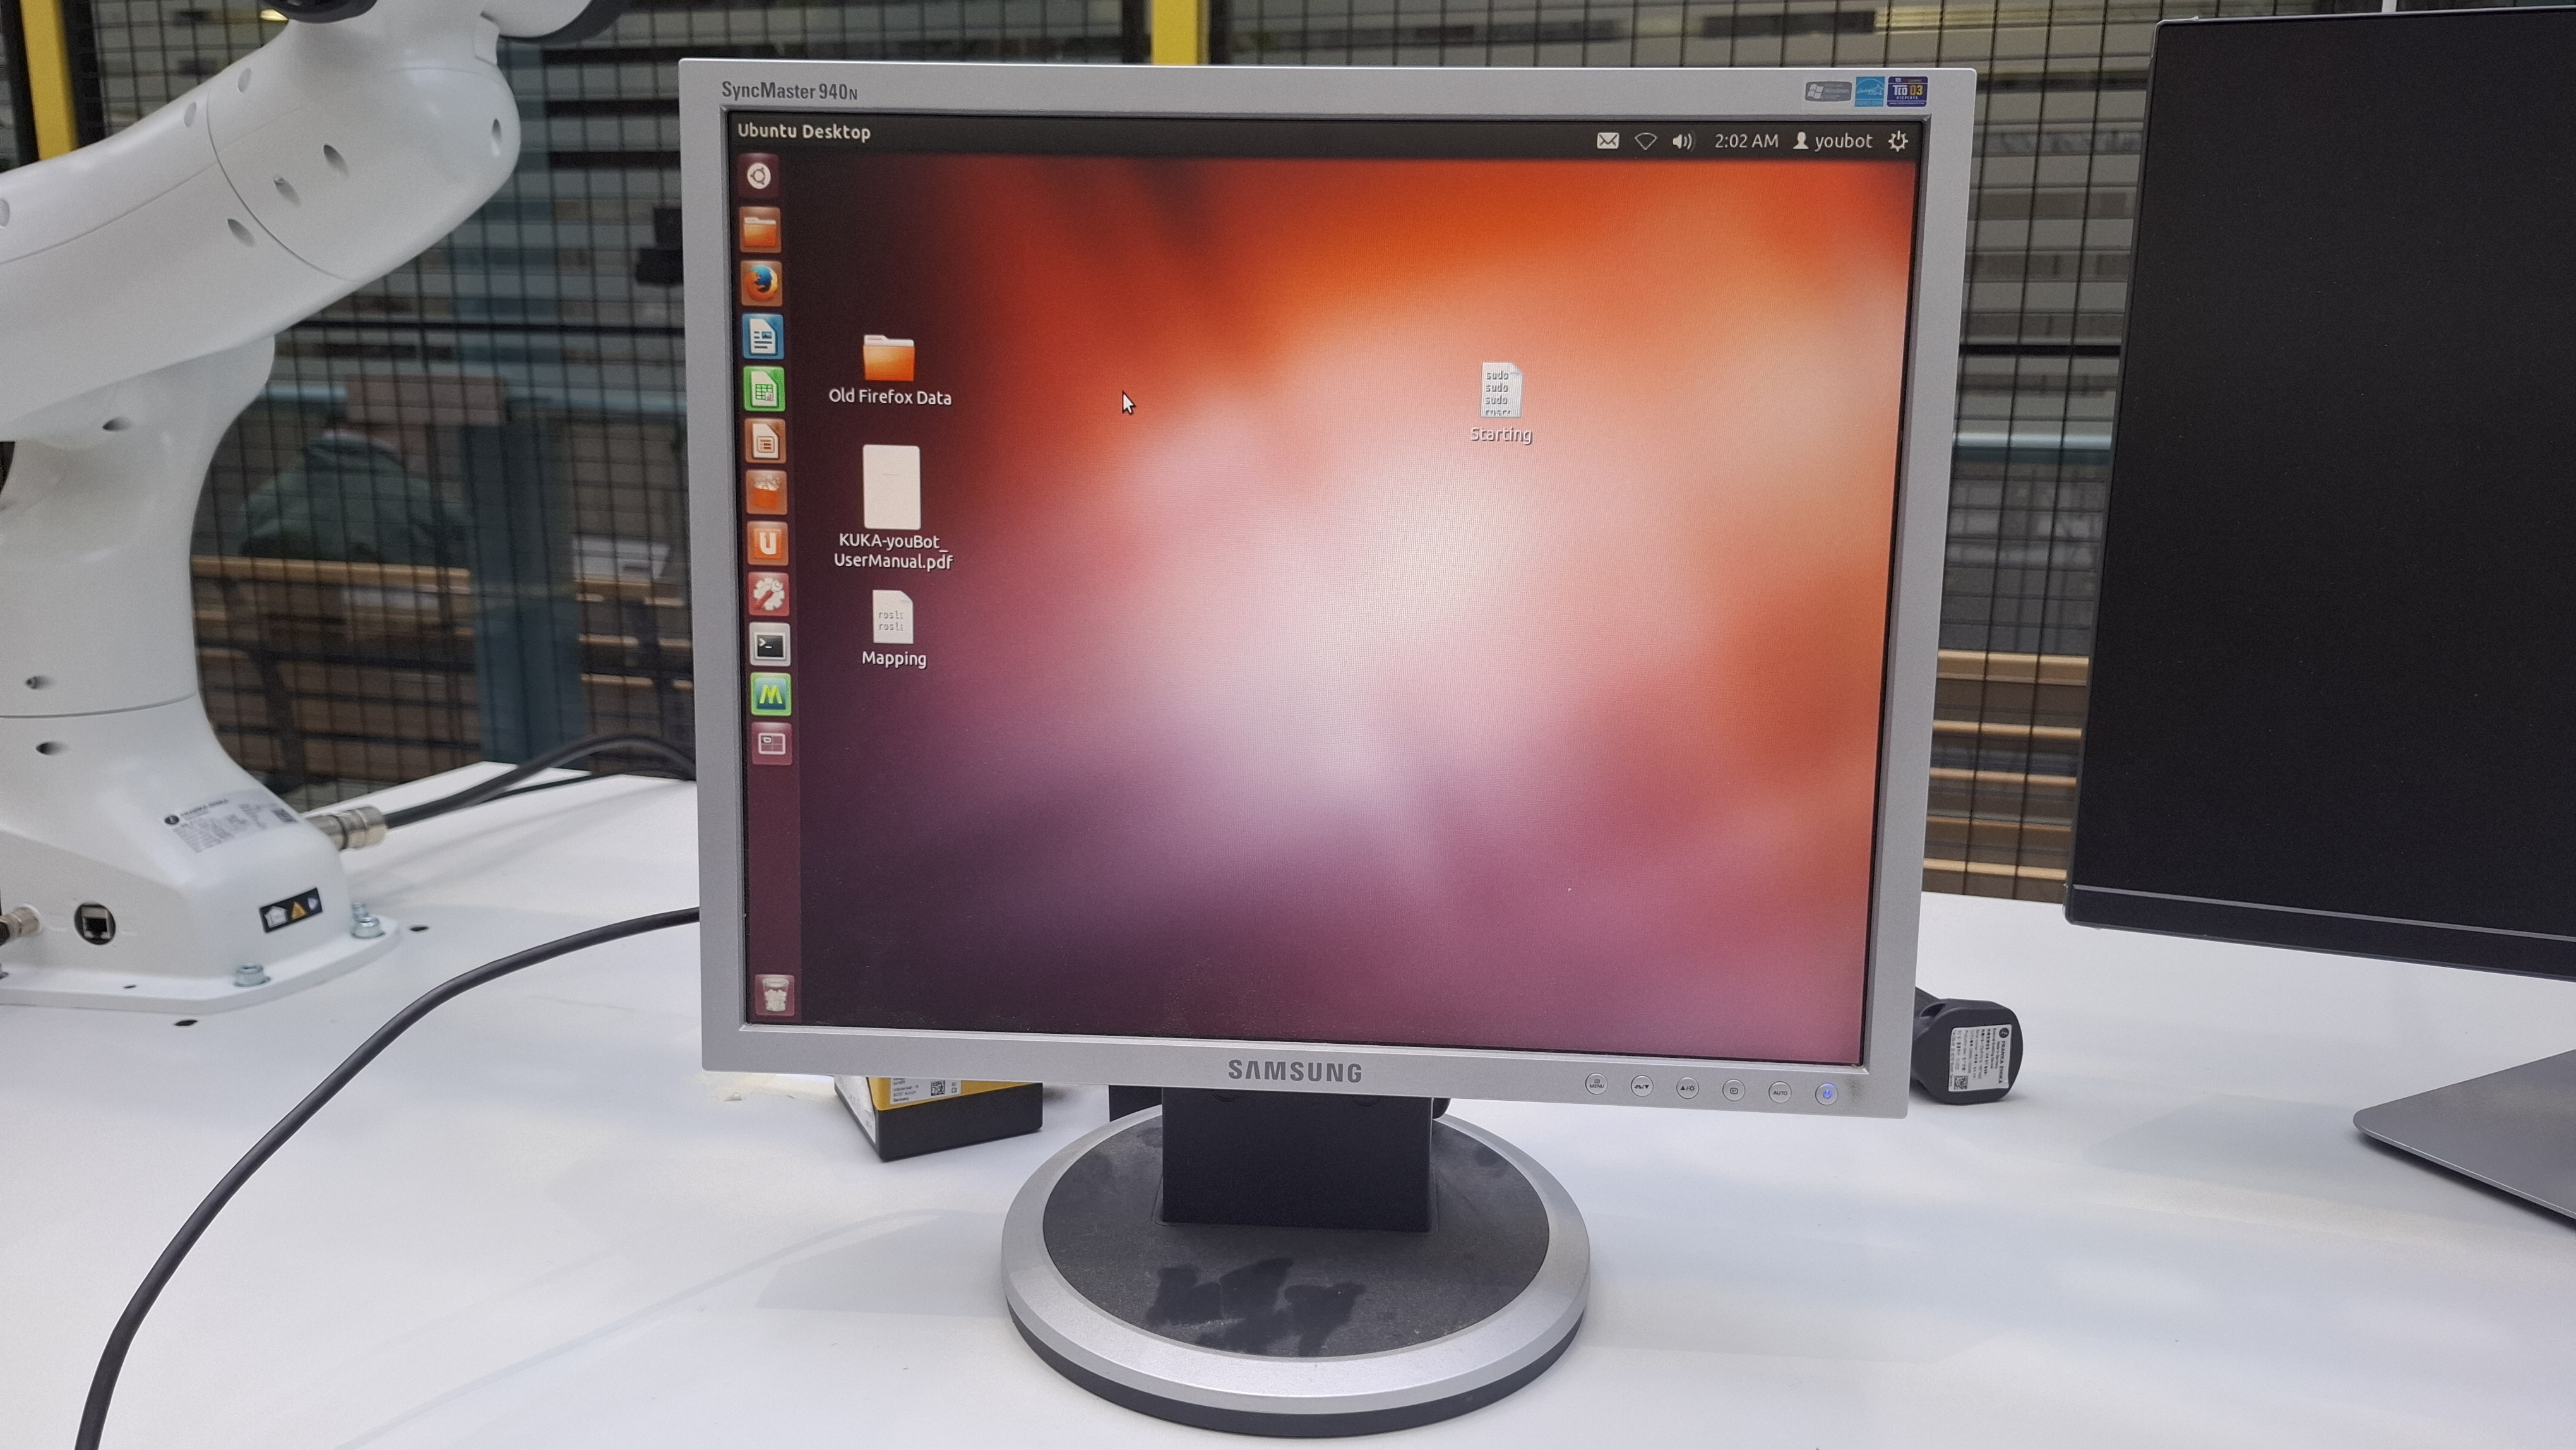
\includegraphics[width=\linewidth]{images/sec4/initial_computer_bootup.jpg}
            \caption{The onboard computer booting up.}
        \end{subfigure}
        \hfill
        \begin{subfigure}[t]{0.49\linewidth}
            \centering
            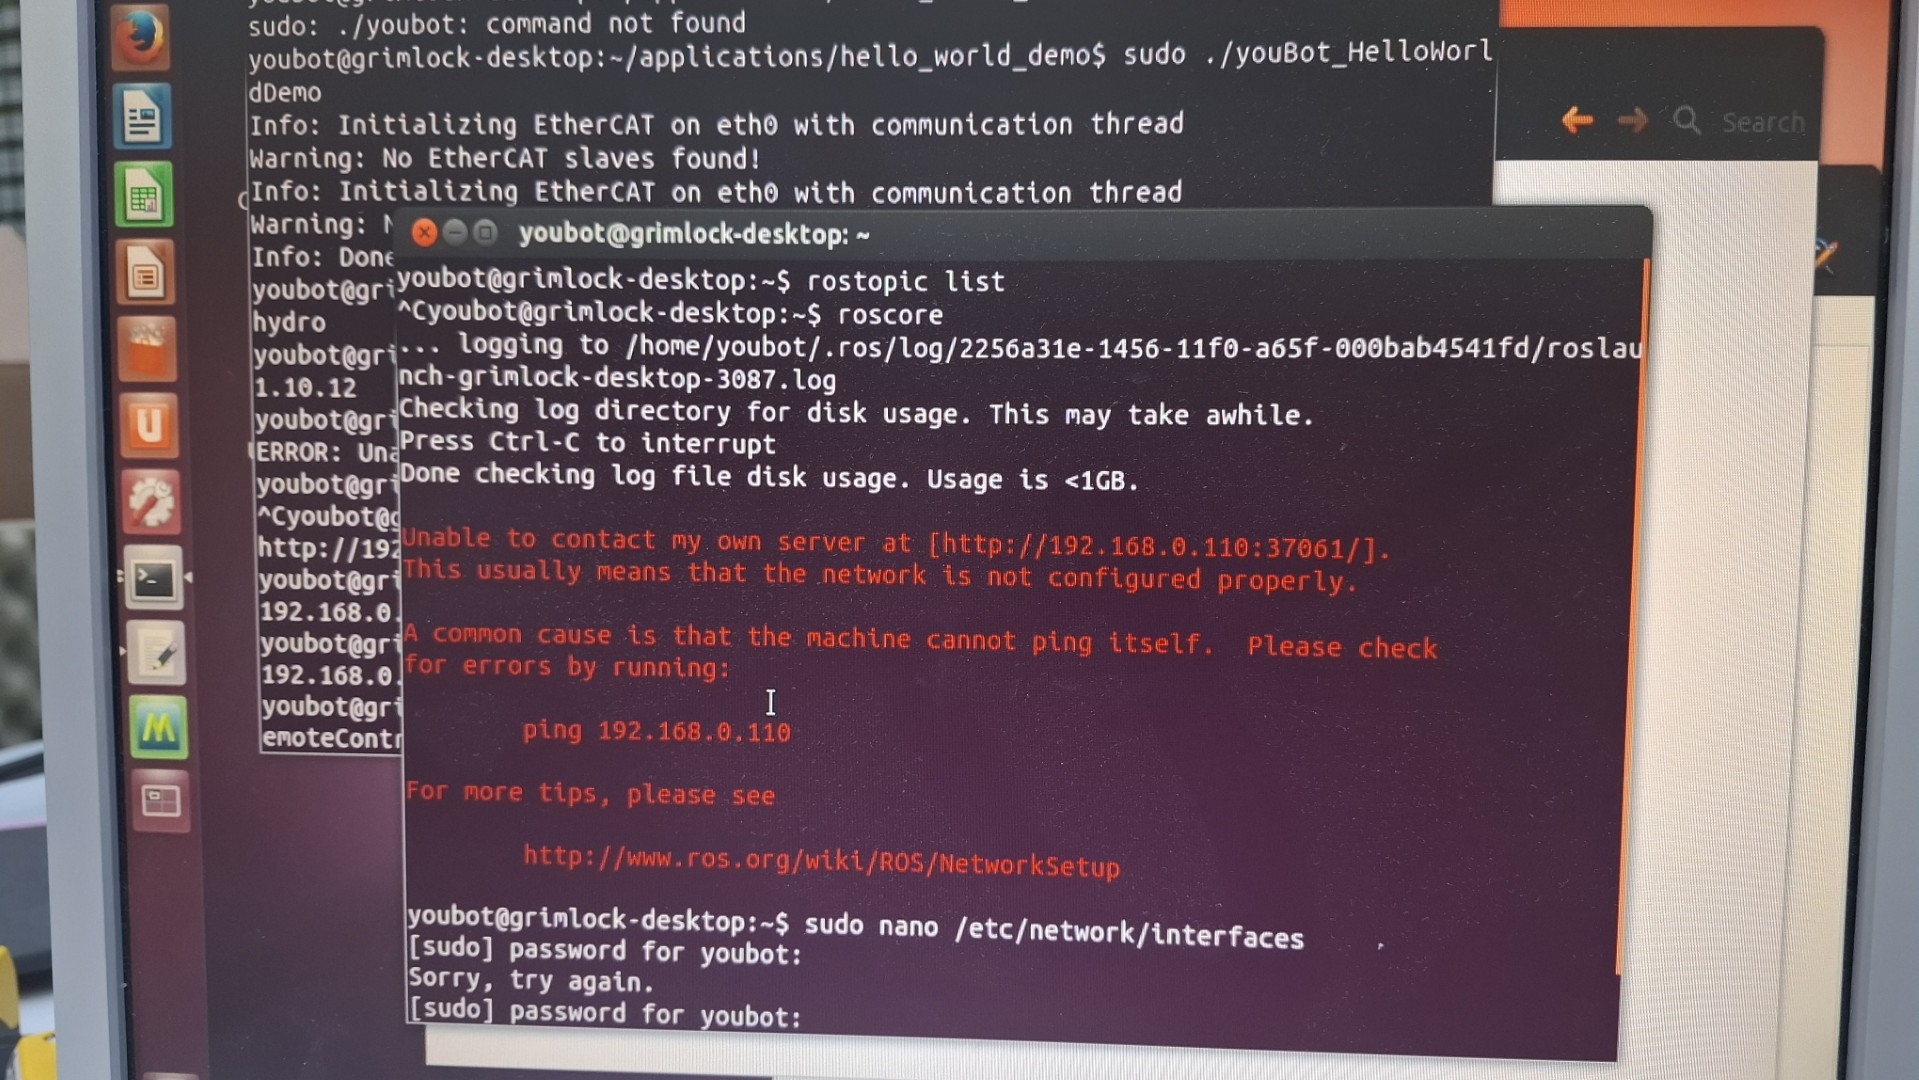
\includegraphics[width=\linewidth]{images/sec4/initial_ros_bootup.jpg}
            \caption{The initial attempt at booting up the ROS interface.}
        \end{subfigure}
        \caption{Initial attempts at booting up the YouBot.}
    \end{figure}

    The ROS interface as well as the relevant demo programs were attempted to be run upon startup without prior configuration. The C++ demo programs were unable to detect any devices on the eth0 port, which was not the port the motors were using. The ROS interface was also unable to ping itself and start \code{roscore}. This was due to the onboard computer not being binded to the correct static IP address, which is necessary for the ROS interface to function properly.

    Furthermore, the onboard computer did not have a static IP address, which meant that it could not be accessed through Ethernet. This would prevent Ethernet-based communication with the YouBot, which would be more reliable than wireless communication. 

    \subsection{Configuration}

    To boot up the C++ programs, the onboard computer required some configuration to suit my current needs. The YouBot config files had to be changed to provide the correct interface (\code{eth1} instead of \code{eth0} for the motors). 

    The Ethernet connection was also configured to use a static IP address, which would allow for reliable communication with the onboard computer. This was done by editing the \code{interfaces} file in the \code{/etc/network/} directory and adding a static IP address for the \code{eth0} interface. 

    After making

    \subsection{C++ demos}

    After configuring the YouBot, I was able to run the C++ demo programs. 

    \subsection{ROS Interface}

    This included changing the \code{.bashrc} file to provide ROS with the correct environment variables, which would in turn allow it to communicate with itself. 

    I was able to start up \code{roscore} after making this change. However, I was not able to run the YouBot-ROS interface due to a lack of permissions to access the \code{eth1} interface. This was due to the fact that the YouBot-ROS interface requires root privileges to access the EtherCAT devices. To resolve this, I had to run the ROS interface with \code{sudo}, which allowed it to access the EtherCAT devices and communicate with the motors. 

    After fixing this issue, I elected to try and run a keyboard teleoperation demo program to test the YouBot's movement capabilities through ROS. This file was stored locally at \code{~/ros_stacks/youbot-ros-pkg/youbot_drivers/youbot_oodl} and could be run by typing:
    \begin{lstlisting}[language=bash]
$    rosrun youbot_oodl youbot_keyboard_teleop.py
    \end{lstlisting}

    I was able to fulfill one of the key project goals, of enabling the YouBot to move through the ROS interface. While there were some issues regarding overcurrent that showed up on some wheels with high speeds, the YouBot was able to move in all directions and turn in place. 

    \subsection{Diving into ROS}

    After getting this to work, my goal now was to understand, at least on a surface level, some of the basic functionalities of ROS, and what nodes and topics the YouBot interface was publishing. Understanding these would enable me to write my own programs to control the YouBot, and to further extend its capabilities. 

    

    

    \subsection{ROS1-ROS2 Bridge}

    One of the first tasks I decided to embark on after getting the robot up and running was to set up the ROS1-ROS2 bridge. This was the most important link within the system, as it would allow the robot to seamless access the ROS2 navigation stack and enable it to access the computational resources of a more recent computer. However, the version of ROS1 on the robot is Hydro, which is more than a decade old and predates ROS2 development, i.e. it is not compatible with a ROS1-ROS2 bridge. 
 
    There are thus a handful of options to consider: One would be to upgrade the ROS1 version of the robot to a version that supports the bridge, such as Melodic or Noetic. However, this would require a significant amount of work and may cause compatibility issues with the outdated software on the robot. Another option would be to use a different computer with a more recent version of ROS1 and use it as a middleware between the robot and the ROS2 navigation stack. This would allow for a more seamless integration of the two systems, but would require additional hardware and software setup and create an unneccesarily complex system. 

    \subsection{Custom Programs}

    I elected to write my own custom programs to control the YouBot, as this would allow me to gain a better understanding of the ROS interface and how to interact with the robot. I started by writing a simple program that would move the YouBot in a square pattern, using the \code{geometry\_msgs/Twist} message type to control the robot's movement. This message type is used to specify the linear and angular velocities of the robot, which can be used to control its movement. 
    

    
    \subsection{Sensors}
    \subsubsection{Kinect Camera and libfreenect}

    The Kinectv1 camera is a depth and RGB camera that was originall designed and sold in tandem with the XBOX 360 to enable motion tracking and gaming. Due to its low cost, high availability and ease of use, it has indirectly become a popular choice for robotics research as well. 

    We can use open-source software such as libfreenect to access the data from the various sensors on the module.


    \notes{discuss the libfreenect library, how to install it, and how it could be used within ROS.}


    \subsubsection{Hokuyo URG-04LX Laser Rangefinder}

    The Hokuyo URG-04LX is a 2D laser rangefinder that is commonly used in robotics research. It is a compact and lightweight sensor that provides high-resolution distance measurements in a 240-degree field of view. The URG-04LX is capable of measuring distances up to 4 meters with an accuracy of +/- 10 mm. It communicates with the onboard computer using a serial interface, making it easy to integrate into existing systems.

    \notes{discuss installing the drivers and whatnot, and how to use it within ROS and rqt.}



    \subsection{Battery Replacement}
    \label{sec:battery-replacement}



    \notes{draft 1, 11.05 12pm\\
    Here are some good web pages about the Slealed Lead Acid (SLA) batteries:
https://batterymasters.co.uk/blog/post/How%20Do%20Sealed%20Lead%20Acid%20Batteries%20Work
and
https://www.power-sonic.com/blog/how-to-charge-a-lead-acid-battery/
and
https://www.powerstream.com/SLA.htm}

    As previously mentioned, the YouBot came with three 24V SLA batteries. Two of these were the original batteries included with the YouBot, and one was a makeshift battery put together by Vesa in 2019. All three batteries were unusable. This section thus documents the technology behind the SLA batteries, the testing of the original batteries, replacing and testing a new battery, and future battery options. 

    \subsubsection{SLA Battery Overview}

    Sealed lead-acid (SLA) batteries operate based on a reversible chemical reaction between lead plates, lead dioxide and sulfuric acid electrolyte. When the battery discharges, the substances react to form lead sultfate and water, releasing electrical energy. During charging, this reaction is reversed.

    These batteries are quite simple, robust, inexpensive and safe to use, indicating the reason for use in this scenario. However, they require some maintainence, and should undergo full discharge and charge cycles regularly to keep them in a good state. If they are not used regularly, they can suffer from sulphation, where lead sulfate crystals gradually form on the plates of the battery. This process is irreversible and permanently impairs the battery's capabilities. Cheaper SLA batteries are more prone to this issue due to lower quality materials, and one may only expect a maximum lifespan of 3-5 years from them. 

    SLA batteries are furthermore sealed and contain one-way valves to prevent internal pressure buildup due to production of hydrogen and oxygen gas. Normally these gases recombine back into water, but overcharging can force gas release, leading in gradual water loss. 

    The recommended voltage for charging SLA batteries is 2.3 volts per cell (2V), or 13.8V for a 6-cell (12V) battery, or 27.6V for a 12-cell (24V) battery. Charging at a lower voltage (i.e. 2V per cell) will not fill up the battery completely, and increase the risk of sulphation, since the lead sulfate crystals will not be fully converted back into active materials. 

    \subsubsection{Testing original batteries}

    To confirm the degradation of the original batteries, we decided to test them using a multimeter. The two original batteries were completely dead, and did not show any voltage when connected to the multimeter. The makeshift battery showed some voltage, but it was far too low to be usable out the gate. This battery was put together using two 12V SLA batteries, where each battery was individually connected to the 4-pin XLR connector. The YouBot internally connects them in series to create a 24V battery.   
    
    Vesa attempted to revive this battery through desulphation, where a higher-than-recommended voltage (in this case, 30V) is applied to the battery to force current through the hardened sulphate layers and dissolve them. 

    This seemed initially promising: the battery was accepting a charge and its voltage was increasing. However, this was only temporary, as the battery quickly lost voltage again after charging, suggesting that the sulphation was very severe. While some surface conductivity was perhaps restored, the effective area of the electrode plates was still very small, resulting in a very low capacity. As such, the battery was not usable for our purposes.  

    \subsubsection{Replacing batteries}

    \notes{maybe here we can link to the specific batteries used? the dimensions would be neat as well...}

    We decided to remake the makeshift battery using two new 12V SLA batteries of the same dimensions. While the previous batteries were Bitelma batteries, we bought some from Leader this time. These batteries were 12V 5.4Ah batteries. We tested them using a multimeter and used a car charger to charge them overnight. 
    
    The old batteries were removed from their casing and all relevant connections and pieces to structure the battery were removed. The new batteries were then appropriately connected to the 4-pin XLR connector \notes{maybe mention the pinout here?}, and the structural pieces were reattached with tape. After putting the casing back on, we were able to connect the new battery to the YouBot and power it on. The YouBot detects the two batteries and shows their individual voltages, confirming that the battery works. While it's not hermetically sealed, it works well for the purposes of this project. 

    \subsubsection{Future Battery Options}

    While we have replaced the SLA batteries with a makeshift one at a rather inexpensive cost, these batteries will not last long and will be prone to the same issues as the original batteries. 

    An ideal candidate for a replacement battery techonology would be lithium-iron-phosphate (LiFePO4) batteries. These batteries are more expensive, but have multiple advantages over SLA batteries. They have longer lifespans, higher energy density, lighter weight, and are less prone to degradation. However, they would also need an integrated battery management system (BMS) to ensure safe operation, and potentially some custom hardware to fit the dimensions of the YouBot's battery compartment. 

    \pagebreak
    
    \section{Experimental Setup for Movement and Odometry}

    There were various inconsistencies that occured during the running of custom programs. For example, the square movement program consistently overshot the expected position with a positive drift in x, y, and yaw. To formally quantify these irregularities, a controlled set of experiments was conducted to assess error rates between actual movement and odometry measurement.


    \subsection{Motivation and Approach}

    The experimental effort was designed to:
    \begin{itemize}[noitemsep]
        \item Quantify the error between commanded and actual movement.
        \item Identify whether errors were consistent (systematic), random, or scale-dependent.
        \item Assess the reliability of onboard odometry over short and long trajectories.
        \item Test how speed and distance affected performance.
        \item Provide insights into feedback control and calibration strategies for error reduction.
    \end{itemize}

    \subsection{Experiment Design}
    A total of 13 experiments were conducted, split into:
    \begin{itemize}[noitemsep]
        \item 5 linear movement tests at different speeds and distances.
        \item 8 rotational movement tests at different speeds and angles.
    \end{itemize}

    Each experiment was carried out 20 times to ensure statistical significance and to allow observation of both deterministic and stochastic error components.

    \subsubsection*{Linear Motion Experiments}

    \begin{table}[H]
    \centering
    \scriptsize
    \begin{tabular}{|c|c|c|}
    \hline
    \textbf{Test ID} & \textbf{Speed (m/s)} & \textbf{Distance (m)} \\
    \hline
    L1 & 0.2 & 1.0 \\
    L2 & 0.4 & 1.0 \\
    L3 & 0.2 & 2.0 \\
    L4 & 0.4 & 2.0 \\
    L5 & 0.6 & 2.0 \\
    \hline
    \end{tabular}
    \caption{Linear motion test configurations}
    \end{table}

    \subsubsection*{Rotational Motion Experiments}

    \begin{table}[H]
    \centering
    \scriptsize
    \begin{tabular}{|c|c|c|}
    \hline
    \textbf{Test ID} & \textbf{Speed (deg/s)} & \textbf{Target Angle} \\
    \hline
    R1 & 45 & 45° \\
    R2 & 75 & 45° \\
    R3 & 45 & 90° \\
    R4 & 75 & 90° \\
    R5 & 45 & 180° \\
    R6 & 75 & 180° \\
    R7 & 45 & 360° \\
    R8 & 75 & 360° \\
    \hline
    \end{tabular}
    \caption{Rotational motion test configurations}
    \end{table}

    \subsubsection{Experimental Procedure}

    The experiments were conducted in a controlled environment on a flat surface. Masking tape was used to make the start and end points of each trajectory, ensuring consistent measurements. The robot then was commanded to move at a specified speed for a calculated duration of time to cover the target distance or angle. The deviation of the final position from the expected position was measured and recorded in a CSV file. Note that for the linear movement tests, the robot center's x and y drift were directly recorded without any additional recordings for the angle deviation, whereas for the rotational movement tests, the x and y drift of two points of the robot (specifically the edge of the middle of the front and back panels) were recorded, and using these data the center of the robot's deviation as well as angle deviation were calculated. 

    \notes{insert diagram here showing how that is done}

    \begin{table}[H]
    \centering
    \scriptsize
    \begin{tabular}{|c|c|c|c|c|c|c|c|}
    \hline
    \textbf{Speed (°/s)} & \textbf{Angle (°)} & \textbf{X Error (m)} & \textbf{Var} & \textbf{Y Error (m)} & \textbf{Var} & \textbf{Yaw Error (°)} & \textbf{Var} \\
    \hline
    45 & 45  & -0.3500 & 0.2525 & -0.6500 & 0.3525 & -7.1310 & 7.4743 \\
    45 & 90  & -0.5750 & 0.5819 &  0.7750 & 0.3119 & -4.8049 & 7.2139 \\
    45 & 180 &  0.5000 & 0.3000 &  0.3000 & 1.3600 & -1.6012 & 9.1212 \\
    45 & 360 &  0.8500 & 0.1275 &  0.2000 & 0.1350 &  7.4315 & 12.4949 \\
    75 & 45  &  0.1000 & 0.1650 & -0.6000 & 0.2900 & -13.3710 & 33.7566 \\
    75 & 90  &  0.4750 & 0.7119 &  0.3500 & 0.4525 & -7.3666 & 34.6317 \\
    75 & 180 &  1.2143 & 0.6565 &  0.7143 & 1.7755 & -5.3584 & 32.1340 \\
    75 & 360 &  1.4500 & 0.3225 &  0.7250 & 1.2119 &  1.8853 & 34.6874 \\
    \hline
    \end{tabular}
    \caption{Rotational motion statistics: Mean error and variance in position (m) and yaw (°)}
    \end{table}

    \begin{table}[H]
    \centering
    \scriptsize
    \begin{tabular}{|c|c|c|c|c|c|}
    \hline
    \textbf{Speed (m/s)} & \textbf{Distance (m)} & \textbf{dx Mean (cm)} & \textbf{dx Var} & \textbf{dy Mean (cm)} & \textbf{dy Var} \\
    \hline
    0.2 & 1 & -4.5500 & 0.2475 &  0.5000 & 1.4500 \\
    0.2 & 2 & -9.0500 & 0.1475 & -0.4500 & 2.9475 \\
    0.4 & 1 & -4.9524 & 0.9025 &  0.8095 & 2.5351 \\
    0.4 & 2 & -9.7000 & 0.8100 & -1.4000 & 10.0400 \\
    0.6 & 2 & -13.3043 & 3.0813 & -20.8261 & 203.5350 \\
    \hline
    \end{tabular}
    \caption{Linear motion statistics: Mean and variance of dx/dy errors (cm)}
    \end{table}



    \begin{figure}[H]
        \centering
        %/flushleft
        %/flushright
        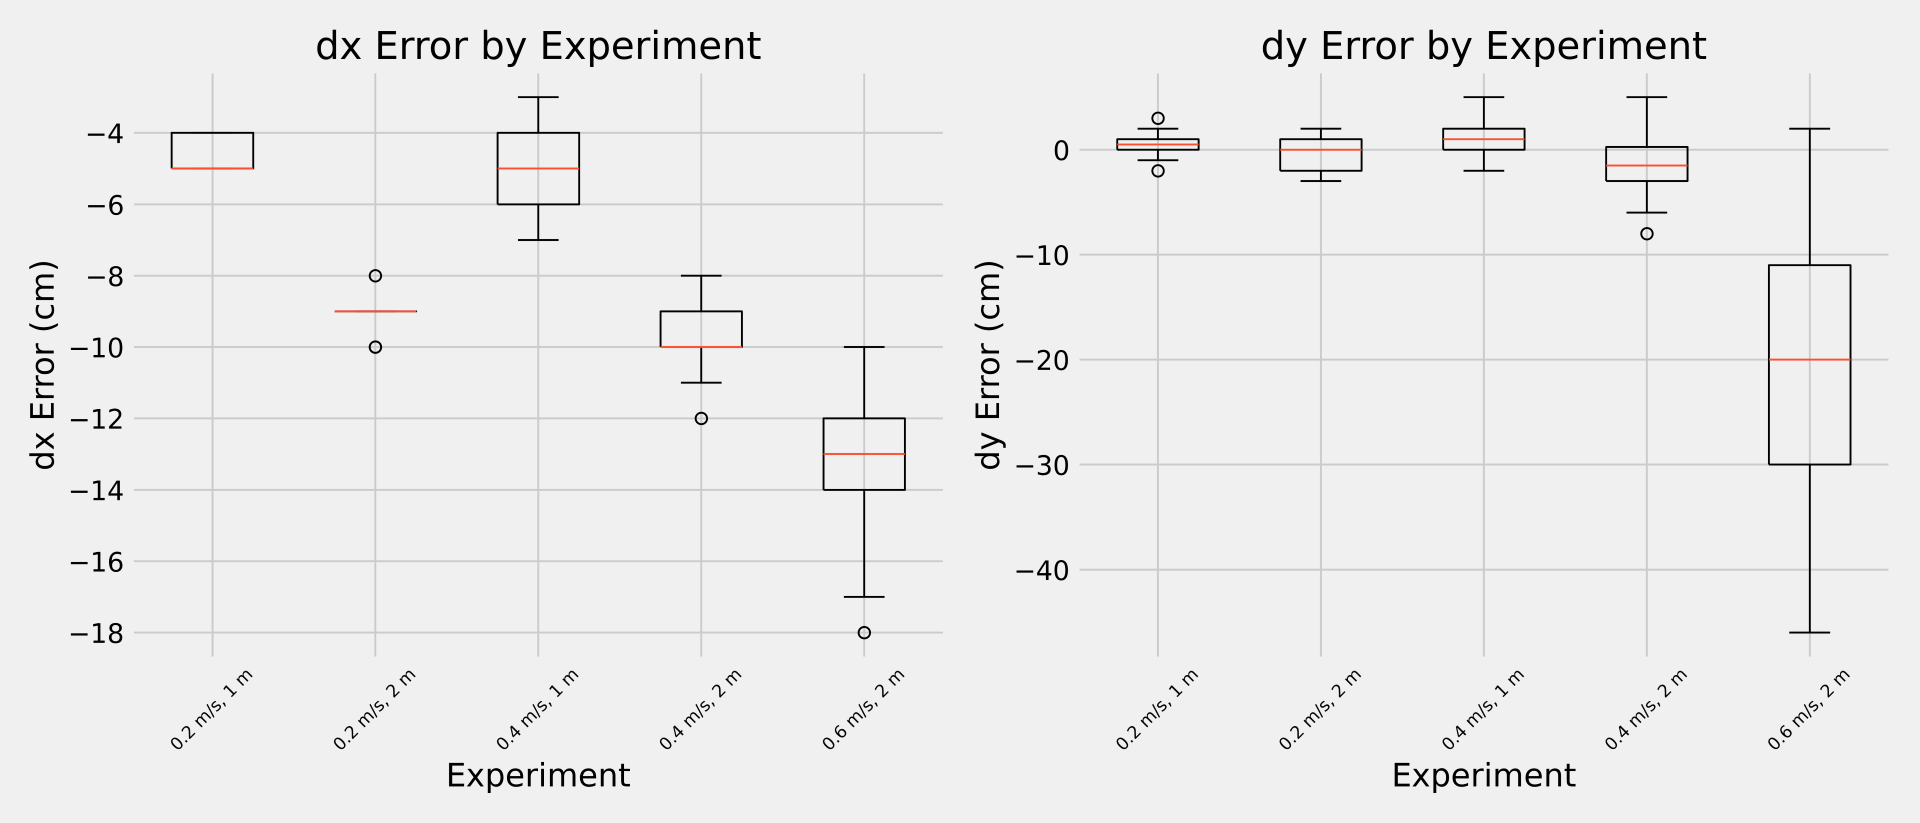
\includegraphics[width=0.99\linewidth]{images/experiment_results/linear_error_boxplots.png}
        \caption{Centered image}
    \end{figure}
    \begin{figure}[H]
        \centering
        %/flushleft
        %/flushright
        
\includegraphics[width=0.99\linewidth]{images/experiment_results/rotational_errors_speed_45.png}
        \caption{Centered image}
    \end{figure}
    \begin{figure}[H]
        \centering
        %/flushleft
        %/flushright
        
\includegraphics[width=0.99\linewidth]{images/experiment_results/rotational_errors_speed_75.png}
        \caption{Centered image}
    \end{figure}

    \subsection{Results and Error Analysis}

    \subsubsection{Linear Motion Error Characteristics}

    The linear motion experiments revealed a consistent underestimation in forward movement (dx), with mean errors increasing approximately linearly with the commanded distance. For instance, at 0.2 m/s over 1 meter, the mean dx error was -4.55 cm, while at 2 meters it was -9.05 cm, indicating a scale-dependent and systematic error. This bias suggests a miscalibration in either velocity estimation or time-based control. In contrast, the lateral error (dy) showed less consistency, with relatively low variance at slow speeds and significantly increased spread at higher velocities (e.g., variance of 203.5 cm² at 0.6 m/s). This may indicate instability in lateral control, sensor drift, or non-ideal surface interactions.

    \subsubsection{Rotational Motion Error Characteristics}

    Rotational experiments exhibited both systematic and random error components. At lower target angles (45° and 90°), yaw error was consistently negative across both speed conditions, pointing to under-rotation. This under-rotation was more severe at higher rotational speeds, suggesting an underestimation of angular displacement due to timing, inertia, or feedback delays. Notably, however, for the 360° trials, the yaw error became positive—indicating over-rotation. This suggests that the error model is nonlinear and possibly affected by controller saturation or feedback lag accumulating over time.

    In addition to yaw deviation, positional drift in x and y was observed during rotation, with the magnitude generally increasing with both angle and speed. For example, at 75°/s over a 360° turn, the mean x and y drift exceeded 1.4 m and 0.72 m respectively. Such drift likely results from an imperfect center of rotation, actuator asymmetry, or encoder discrepancies.

    \subsubsection{Classification of Errors}

    Based on the data, errors were classified as follows:
    \begin{itemize}
        \item \textbf{Systematic Errors:} Present in both dx and yaw measurements. These were repeatable and dependent on motion parameters, suggesting calibration issues or consistent model inaccuracies.
        \item \textbf{Random Errors:} Particularly visible in dy and yaw variance, especially at higher speeds. These may arise from environmental factors, surface inconsistencies, or sensor noise.
        \item \textbf{Scale-Dependent Errors:} Errors in dx and yaw tended to grow with increasing speed and commanded magnitude, indicating drift or temporal misalignment in control commands.
        \item \textbf{Nonlinear and Saturation Effects:} Reversal of yaw error direction (under-rotation to over-rotation) at large angles and high speeds suggests complex behavior beyond linear drift, potentially due to limits in the control loop or cumulative errors in open-loop motion.
    \end{itemize}

    These results underscore the need for either closed-loop feedback or more accurate modeling of motion and sensor characteristics to reduce the observed deviation, especially for longer or faster movements. 

    \pagebreak

    \section{Future Applications}

    While the Teach and Repeat (T\&R) method---a form of visual SLAM where the robot is manually guided through a path and then repsereats it using stored visual keyframes---has been applied in robotics, its real-world utility on the KUKA YouBot is nuanced. The platform is best viewed not as an ideal assistive robot for dynamic human environments, but as a robust mobile base for prototyping, logistics, and structured automation tasks.

    \subsection{Platform Considerations}

    The YouBot, with its omnidirectional drive and compact form, offers a flexible and extensible base. However, its limited onboard compute and sensing make it suboptimal for tasks requiring high adaptability or semantic awareness---both critical for assistive service robots in real homes or public environments. Nonetheless, its utility in controlled or semi-structured settings remains strong.

    \subsection{Practical Deployment Context}

    In the broader context of mobile robot deployment, there are three major paradigms:

    \begin{itemize}[noitemsep]
        \item \textbf{Infrastructure-Dependent AGVs:} Traditional automated guided vehicles rely on pre-installed infrastructure such as reflector stripes or magnetic paths. These are effective in fixed-route logistics (e.g., forklift automation in warehouses), but require significant setup and cannot adapt dynamically.
        \item \textbf{Smart AMRs:} Autonomous mobile robots (like those used by Amazon) can replan paths in real-time using onboard sensors and cloud coordination. These systems excel in semi-structured logistics environments with moving agents and dynamic layouts.
        \item \textbf{Grid-Based Swarm Platforms:} Some warehouse systems use fleets of robots operating on a grid, optimizing item retrieval and packing through centralized orchestration (e.g., AutoStore systems). These prioritize high efficiency in tightly structured environments.
    \end{itemize}

    \subsection{Potential Roles for the YouBot Base}

    While not competitive with fully integrated AMRs or commercial AGVs, the YouBot base can serve as a:

    \begin{itemize}[noitemsep]
        \item \textbf{Flexible Intra-Logistics Tool:} Ideal for transporting light items within labs or workshops in predefined or moderately dynamic spaces.
        \item \textbf{Assistive Demonstrator:} For fetching or guiding in controlled environments (e.g., academic demos, elderly care labs).
        \item \textbf{Research Platform:} Excellent for testing navigation, mapping, and multi-agent systems thanks to its ROS compatibility and open interfaces.
        \item \textbf{Educational Robot:} Its small footprint and programmability make it a staple in teaching and competitions.
    \end{itemize}

    \subsection{On the Use of Teach and Repeat}

    T\&R may still be useful in scenarios where:

    \begin{itemize}[noitemsep]
        \item The environment is static and predictable.
        \item The path is repetitive (e.g., lab-to-lab delivery).
        \item The focus is on rapid prototyping of navigation methods with minimal setup.
    \end{itemize}

    However, for adaptive assistive platforms, T\&R lacks the semantic and reactive capabilities necessary to operate alongside humans in dynamic contexts.

    \subsection{Summary Table}

    \begin{table}[H]
    \centering
    \begin{tabular}{|l|p{7cm}|}
    \hline
    \textbf{Application Area} & \textbf{Role of YouBot} \\
    \hline
    Intra-logistics & Automating small transport tasks in labs/factories \\
    Assistive robotics (demonstrator) & Simple delivery/fetching in structured indoor environments \\
    Research and prototyping & Platform for SLAM, navigation, and HRI testing \\
    Education and training & Robotics coursework, student projects, competitions \\
    \hline
    \end{tabular}
    \caption{Summary of Practical Applications for the KUKA YouBot Base}
    \end{table}


    


    \pagebreak

    \section{Reflection}

    \notes{draft 1, 11.05 6pm}

    In this section, I will reflect on the outcomes of this project. This will include an overview of project management practices and planning, alongside my learnings and personal feelings about the project. 

    \subsection{Project Evolution}

    As disccused previously, the initial goal of this project was much more concrete and ambitious, with an ultimate aim of enabling Teach and Repeat on a decade-old robot whilst using something like ROS2 Jazzy. This was simply not feasible with the outdated software and hardware, lack of documentation, my own lack of experience, and the overall time and resource constraints for completing this project. Furthermore, this project was a significant different experience from any other course I have taken in the past.
    
    My initial approach to project management was very linear and straighforward, with the understanding that there would be no hiccups or issues along the way. I had the following time-table in mind: \notes{maybe insert a table showcasing the plan here?} While this was initially rewarding as I made progress in individual tasks (i.e. Kinect camera, booting up computer, static IP, etc.), momentum was quickly lost when it came to integrating these tasks into a cohesive system, through the use of the ROS1-ROS2 bridge. 

    \subsection{AGILE}

    The new mindset I undertook was inspired by the AGILE project management methodology, which takes a much more flexible and iterative approach to project management. While the long-term goals are still important, the focus is on short-term goals and iterations. This allows for a more flexible approach, where the ending goal can be adjusted based on constraints, feedback, and progress. 

    While this also indirectly means that the project may not be concretely completed, it led to a more flexible exploration of the robot's capabilities and limitations. It furthermore relieved me of the pressure of having to complete a specific (and steep) goal, and gave me breathing space to play around with the available components more freely. This was much more rewarding and enjoyable.

    Undertaking this mindset required time and patience, where I had to learn to accept that not everything would go according to plan. It furthermore required me to be more open to feedback, and actively focusing on short-term goals. 

    \subsection{Final Thoughts}

    Overall, despite the various challenges faced, I am very happy with my progress and learning outcomes regarding this project. I was able to successfully revive the KUKA YouBot to a usable state, gain a deeper understanding of the ROS ecosystem, Linux, bash scripting, alongside the various hardware components of the robot. More importantly, I learned to manage projects with the understanding of personal and technical constraints. I'd like to thank my advisor for his provision of a different perspective on the project, explanations of everything and constant patience.  


    \newpage

    \printbibliography

    \newpage

    \appendix


    \section{User Manual for the KUKA YouBot}

    \subsection{Booting Up the YouBot}
    To begin operating the YouBot, follow these steps to power up the system and access the onboard computer interface using a monitor and peripherals. 

    \subsubsection{Powering On}
    \begin{enumerate}[topsep=0pt, noitemsep]
        \item Plug the YouBot into a power source using the provided power cable and adapter through the top panel. Ensure that the supply voltage is compatible (24V DC).
        \item Press the main power button located on the top panel of the YouBot. This will power the system on. Note that the onboard computer and motors are not powered on by default. 
        \item Connect a monitor using the provided VGA port. Note that this is required to be plugged in before powering on the YouBot, as the onboard computer will not boot up with a GUI otherwise. 
        \item Turn the onboard computer and motors on. Long press the power button to cycle through options for powering the subsystems. Toggle by releasing the button when the desired option is highlighted. 
        \item Wait for the onboard computer to boot up. This may take a few minutes. 
        \item Plug in USB peripherals such as a keyboard and mouse to interact with the onboard computer.
        \item Once the computer has booted, you should see a desktop environment similar to a standard Linux distribution. You can now interact with the onboard computer using the keyboard and mouse. Note that the default credentials are: 
        \begin{itemize}[topsep=0pt, noitemsep]
            \item Username: \code{youbot}
            \item Password: \code{youbot}
        \end{itemize}
    \end{enumerate}

    \notes{add image of the booting up process.}

    \subsection{Initial Configuration}

    After booting up the YouBot, some initial configuration is required to enable the ROS interface and the YouBot drivers. This includes setting up the ROS networking configuration, configuring the Ethernet interface, and editing the YouBot driver configuration file. 

    \subsubsection{ROS Networking Configuration (\code{.bashrc})}
    Update the onboard computer's \code{.bashrc} file with the following: 

    \begin{lstlisting}[style=plain]
    export MY_IP=localhost

    export ROS_IPV6=off
    export ROS_HOSTNAME=$MY_IP
    export ROS_MASTER_URI=http://$MY_IP:11311
    export ROS_IP=$MY_IP

    export ROS_PACKAGE_PATH=$ROS_PACKAGE_PATH://home/youbot/youbot_driver:/home/youbot/ros_stacks:/home/youbot/applications
    export LIBGL_ALWAYS_SOFTWARE=1

    source /opt/ros/hydro/setup.bash
    \end{lstlisting}
%    source ~/DSD/devel/setup.bash #this will be covered later.

    To verify configuration:
    \begin{lstlisting}[style=plain]
$   roscore 
    \end{lstlisting}

    %This will set the ROS networking configuration to use the local host as the IP address, and will ensure that the ROS interface can communicate with itself. The \code{ROS_PACKAGE_PATH} variable is also set to include the necessary directories for the YouBot drivers and applications. To test whether ROS is now able to communicate with itself, the following command was run:

    %If the command runs successfully, it means that the ROS interface is now able to communicate with itself and is ready to be used. 

    \subsubsection{Ethernet Configuration (\code{/etc/network/interfaces})}

    To enable stable communication between the YouBot and external systems, a static IP address is preferably assigned to the onboard Ethernet interface. This enables reliable wired access for remote control. 

    \textbf{ote:} Not all Linux distributions name Ethernet interfaces as \code{eth0}, and instead may use interfaces named \code{eth1}, \code{enp2s0}, etc. To identify the correct interface, use the following command:

    \begin{lstlisting}[style=plain]
$   ip link show
    \end{lstlisting}

    Look for an interface name associated with a physical Ethernet port. In the following instructions, replace \code{eth0} with the appropriate interface name.
    
    Assign a permanent static ethernet IP by editing the file \code{/etc/network/interfaces} and adding:

    \begin{lstlisting}[style=plain]
    auto eth0
    iface eth0 inet static 
        address 192.168.10.1            ## The static IP address to be assigned
        netmask 255.255.255.0           ## Standard subnet mask
    \end{lstlisting}

    Replace \code{eth0} with your actual interface name as determined above. Save the file and apply changes:

    \begin{lstlisting}[style=plain]
$   sudo /etc/init.d/networking restart
    \end{lstlisting}

    Confirm the static IP assignment by checking the interface configuration:
    \begin{lstlisting}[style=plain]
$   ip addr show eth0
    \end{lstlisting}


   \textbf{Note:} An alternative to an Ethernet configuration is to assign a static IP via the network router on a wireless interface. This eliminates a wired connection dependency and allows the YouBot to obtain a static IP automatically when connected to the same network. Refer to your router's documentation for specific instructions on conducting DHCP reservations. 

    \paragraph{Testing the Connection}
    After configuration, connect another device (e.g., a laptop) to the YouBot via Ethernet. Assign the other device a static IP in the same subnet (e.g., \code{192.168.10.2}). Then test connectivity:

    \begin{lstlisting}[style=plain]
    $ ping 192.168.10.1         ## From the laptop to the YouBot
    \end{lstlisting}

    For remote terminal access:

    \begin{lstlisting}[style=plain]
    $ ssh youbot@192.168.10.1
    \end{lstlisting}

    Enter the password when prompted (default is \code{youbot}). If the connection is successful, the YouBot should be accessible through an external PC. 


    \subsubsection{Youbot Driver Configuration (\code{~/youbot_driver/config/youbot-ethercat.cfg})}

    The YouBot driver requires the correct Ethernet interface to be specified for EtherCAT communication with the base and arm motors. This is configured in the file \code{~/youbot_driver/config/youbot-ethercat.cfg}. Note that the interface name used here may be different from the Ethernet interface name used in the previous step.  Type the following to see your Ethernet interfaces:
    \begin{lstlisting}[style=plain]
$   ifconfig
    \end{lstlisting}

    Change the Ethernet interface name in the youbot configuration file \\(\code{~/youbot_driver/config/youbot-ethercat.cfg}) to match your actual interface name:

    \begin{lstlisting}[style=plain]
    #EtherCAT port
    [EtherCAT]
    EthernetDevice = eth1 # Change this to your actual EtherCAT interface name
    \end{lstlisting}

    This will enable the YouBot driver to communicate with the motors and sensors through the correct port for the C++ demos. Run and test either the C++ demos or the ROS interface to verify that the configuration is correct. 


    
    \subsection{Running C++ demos}

    \textbf{Note:} Remember to turn the motors on before running the demos. This can be done by long-pressing the power button on the top panel of the YouBot and toggling the "Motors" option to ON.

    The YouBot provides precompiled C++ demo applications located in \code{~/applications}. These are also available from the official \code{youbot_applications} GitHub repository. The demos include basic tests for motor communication and manual control interfaces.

    \subsubsection{Hello World Demo}

    This demo verifies that the EtherCAT communication is working correctly by issuing movement commands to the robot.

    To run it:

    \begin{lstlisting}[style=plain]
    $ cd ~/applications/hello_world_demo/bin
    $ sudo ./youBot_HelloWorldDemo
    \end{lstlisting}

    If successful, the output will indicate that the application is connected to the motors, and the robot should briefly move in the four cardinal directions (forward, backward, left, and right), confirming functional motor control.

    \subsubsection{Keyboard Control Demo}

    This demo enables basic manual control of the YouBot using the keyboard. It allows testing of real-time responsiveness and manual teleoperation.

    Run it with:

    \begin{lstlisting}[style=plain]
    $ cd ~/applications/keyboard_control_demo/bin
    $ sudo ./youBot_KeyboardControlDemo
    \end{lstlisting}

    Use the on-screen instructions to control the robot’s movement via the keyboard. 

    One may run the other demos in a similar manner. Refer to the GitHub repository's README for more details. 

    \subsection{Running the ROS Interface}

    Once the C++ demos have been confirmed functional, the ROS (Robot Operating System) interface can be used to enable modular software integration for motion planning, visualization, diagnostics, and teleoperation.

    \subsubsection{Verifying Installed ROS Packages}

    To verify the required packages are installed on the YouBot, run:

    \begin{lstlisting}[style=plain]
    $ rospack list
    \end{lstlisting}

    Ensure the following packages are present:

    \begin{itemize}[topsep=0pt, itemsep=0pt]
    \item \code{youbot_driver_ros_interface} – Core ROS hardware interface for the YouBot.
    \item \code{youbot_teleop} – ROS node for keyboard-based teleoperation.
    \item \code{youbot_common} – Common message definitions and configuration files.
    \item \code{youbot_description} – URDF robot model and related assets.
    \end{itemize}

    \subsubsection{Launching the ROS Driver}

    Before launching the ROS interface, ensure the correct environment variables are set (see section: \textit{ROS Networking Configuration}). Then launch the ROS master and the YouBot driver:

    \begin{lstlisting}[style=plain]
    $ roscore
    $ roslaunch youbot_driver_ros_interface youbot_driver.launch
    \end{lstlisting}

    The driver initializes the EtherCAT interface and exposes the robot's hardware components to the ROS environment.

    \subsubsection{Inspecting Nodes and Topics}

    Use the following commands to inspect active ROS nodes and topics:

    \begin{lstlisting}[style=plain]
    $ rosnode list
    $ rostopic list
    \end{lstlisting}

    Example nodes:

    \begin{itemize}[topsep=0pt, itemsep=0pt]
    \item \code{/youbot_driver} – Node that manages all hardware-level communication.
    \item \code{/rosout} – Default ROS logging node.
    \end{itemize}

    Example topics:

    \begin{itemize}[topsep=0pt, itemsep=0pt]
    \item \code{/joint_states} – Publishes joint positions and velocities.
    \item \code{/cmd_vel} – Accepts velocity commands for the base.
    \item \code{/tf} – Publishes coordinate frame transforms.
    \end{itemize}

    \subsubsection{Using Visualization Tools: \code{rqt} and \code{rviz}}

    ROS visualization tools are used to monitor system behavior and robot state:

    \begin{itemize}[topsep=0pt, itemsep=0pt]
    \item \code{rqt_graph} – Displays real-time node and topic communication graph.
    \item \code{rviz} – Visualizes robot model, coordinate frames, sensor data, and state feedback.
    \end{itemize}

    Run the following commands in separate terminals:

    \begin{lstlisting}[style=plain]
    $ rosrun rqt_graph rqt_graph
    $ rosrun rviz rviz
    \end{lstlisting}

    
    \subsection{Writing Custom Programs}

    This section describes how to create and run custom ROS programs to control the YouBot using Python. The provided ROS demo packages serve as a reference.

    \subsubsection{Creating a Catkin Workspace}

    Before writing custom ROS programs, create a Catkin workspace to manage packages and dependencies. Note that we have named our folder \code{DSD} to reflect the course name. 

    \begin{lstlisting}[style=plain]
    $   mkdir -p ~/DSD/catkin_ws/src 
    $   cd ~/DSD/catkin_ws/
    $   catkin_make
    \end{lstlisting}

    Source the workspace to update your ROS environment:

    \begin{lstlisting}[style=plain]
    $ source devel/setup.bash
    \end{lstlisting}

    To source automatically in every new terminal, add this line to your \code{.bashrc}:

    \begin{lstlisting}[style=plain]
    echo "source ~/DSD/catkin_ws/devel/setup.bash" >> ~/.bashrc
    \end{lstlisting}

    \subsubsection{Creating a Custom Package}

    Create a new ROS package named \code{youbot_control} with dependencies:

    \begin{lstlisting}[style=plain]
    $ cd ~/DSD/catkin_ws/src
    $ catkin_create_pkg youbot_control rospy std_msgs geometry_msgs # youbot_control is the package name, the following are dependencies
    $ cd ~/DSD/catkin_ws
    $ catkin_make
    \end{lstlisting}

    \subsubsection{Writing a Python Control Script}

    Inside your package directory, create a \code{scripts} folder and a Python control script:

    \begin{lstlisting}[style=plain]
    $ cd ~/DSD/catkin_ws/src/youbot_control
    $ mkdir scripts
    $ touch scripts/simple_move.py
    $ chmod +x scripts/simple_move.py # Make the script executable
    \end{lstlisting}

    Sample code files can be found in \notes{appendix for code}

    To run a script:

    \begin{lstlisting}[style=plain]
    $ rosrun youbot_control simple_move.py
    \end{lstlisting}

    \textbf{Note:} Note that certain scripts require additional arguments to be passed in. Refer to the comments for details. 

    \subsubsection{Automation with Bash Scripts and Tmux}

    Manually opening multiple terminals and running ROS nodes is tedious. This process can be automated using a combination of bash scripts and \code{tmux}.

    First, install \code{tmux} if not already available:

    \begin{lstlisting}[style=plain]
    $ sudo apt-get install tmux
    \end{lstlisting}

    Then, create a bash script to launch the environment in multiple panes:

    \begin{lstlisting}[style=plain]
    $ touch launch_youbot.sh
    $ chmod +x launch_youbot.sh
    \end{lstlisting}

    Sample content for \code{launch_youbot.sh} can be found in \notes{appendix for code}. This script will create a new \code{tmux} session with three panes: one for \code{roscore}, one for the YouBot driver, and one for a custom movement script. Run the script by navigating to its directory and running the command:

    \begin{lstlisting}[style=plain]
    $ ./launch_youbot.sh 
    \end{lstlisting}

    Note that a password will be required to initialize the YouBot-ROS interface. Navigate between panes using \code{Ctrl+b} followed by the arrow keys. Detach from the session with \code{Ctrl+b d} and reattach later with:
    \begin{lstlisting}[style=plain]
    $ tmux attach-session -t youbot
    \end{lstlisting}
    
    Refer to the \code{tmux} documentation for more advanced usage and commands.

    \subsubsection{Using TMuLE for Configuration Management}

    One may use TMuLE to simplify the scripting process further using toml files. The youbot did not allow for the installation of TMuLE due to no support for Python 2.7, so this was not used in this project. However, it is a useful tool to consider for future projects. Refer to the documentation here. 
   
    \pagebreak
    \section{Code files}
    %\lstinputlisting[language=Python, caption={Full Script}, label={lst:fullscript}]{../code/rotate_graph.py}
    \subsubsection{rotate\_graph.py}
    This script read the data collected from the rotational movement experiments to parse the data and plot the drift of the centre of the robot in x and y axes as well as difference in yaw in a graph format. It also prints out the mean and standard deviation of the relevant errors. Refer to \notes{insert something here idr} for further details. 
    \lstinputlisting[language=Python, label={lst:fullscript}]{../code/rotate_graph.py}
    \pagebreak
    \subsubsection{linear\_graph.py}
    This script read the data collected from the linear movement experiments to parse the data and plot the drift of the centre of the robot in x and y axes in a graph format. It also prints out the mean and standard deviation of the relevant errors. Refer to \notes{insert something here idr} for further details. 
    \lstinputlisting[language=Python, label={lst:fullscript}]{../code/linear_graph.py}
    \pagebreak
    \subsubsection{linear\_test.py}
    This script is used to undertake the linear movement experiments. It uses the ROS interface to send velocity commands to the YouBot, and then calculates the delta in odometry from the robot. The script is designed to be run multiple times with different parameters through the terminal to collect data for analysis. Refer to \notes{insert something here idr} for further details.
    \lstinputlisting[language=Python, label={lst:fullscript}]{../code/youbot-files/DSD/src/youbot_control/scripts/linear_test.py}
    \pagebreak
    \subsubsection{rotate\_test.py}
    This script is used to undertake the linear movement experiments. It uses the ROS interface to send velocity commands to the YouBot, and then calculates the delta in odometry from the robot. The script is designed to be run multiple times with different parameters through the terminal to collect data for analysis. Refer to \notes{insert something here idr} for further details.
    \lstinputlisting[language=Python, label={lst:fullscript}]{../code/youbot-files/DSD/src/youbot_control/scripts/rotate_test.py}
    \pagebreak
    \subsubsection{simple\_square\_movement.py}
    This script was used to test the YouBot's ability to move in a square pattern. It uses the ROS interface to send velocity commands to the YouBot. 
    \lstinputlisting[language=Python, label={lst:fullscript}]{../code/youbot-files/DSD/src/youbot_control/scripts/simple_square_movement.py}
    \pagebreak
    \subsubsection{Tmux automation script} 
    This script is used to automate the process of launching the ROS interface and the custom control scripts in a tmux session. It creates a new tmux session with four panes: one running \code{the YouBot-ROS interface}, one running the keyboard controller node, and two free panes for miscellaneous purposes.
    \lstinputlisting[language=Bash, label={lst:fullscript}]{../code/youbot-files/DSD.sh}

    \pagebreak


    \section{Experimental Data}

    \subsection{Linear movement experiment}
    \subsubsection{Linear movement, 0.2m/s, 1m}
    \begin{table}[H]
    \scriptsize
    \begin{tabular}{@{}cccccc@{}}
    \toprule
    \textbf{dx\_meas} & \textbf{dy\_meas} & \textbf{dx\_odom} & \textbf{dy\_odom} & \textbf{dz\_odom} & \textbf{dyaw\_odom} \\ \midrule
    100          & -4           & 96       & -1       & 0        & -0.012     \\
    103          & -2           & 98       & -2       & 0        & -0.012     \\
    102          & -1           & 98       & -3       & 0        & 0.003      \\
    99           & 0            & 95       & -1       & 0        & -0.006     \\
    102          & -2           & 98       & 0        & 0        & -0.013     \\
    100          & -1           & 95       & 0        & 0        & -0.001     \\
    102          & -1           & 98       & 0        & 0        & 0.005      \\
    103          & -2           & 98       & 0        & 0        & 0.005      \\
    104          & -1           & 99       & -1       & 0        & 0.006      \\
    102          & -2           & 97       & 0        & 0        & -0.004     \\
    103          & 0            & 98       & 0        & 0        & -0.010     \\
    104          & -1           & 99       & -1       & 0        & 0.003      \\
    102          & -1           & 98       & -1       & 0        & 0.004      \\
    102          & 0            & 97       & 0        & 0        & 0.002      \\
    100          & 0            & 96       & -1       & 0        & 0.012      \\
    103          & -1           & 98       & 0        & 0        & 0.007      \\
    103          & -1           & 98       & 0        & 0        & 0.003      \\
    100          & -1           & 96       & 0        & 0        & 0.004      \\
    100          & -1           & 96       & 0        & 0        & -0.003     \\
    103          & 0            & 98       & -1       & 0        & 0.008      \\ \bottomrule
    \end{tabular}
    \end{table}

    \subsubsection{Linear movement, 0.2m/s, 2m}
    \begin{table}[H]
    \scriptsize
    \begin{tabular}{@{}cccccc@{}}
    \toprule
    \textbf{dx\_meas} & \textbf{dy\_meas} & \textbf{dx\_odom} & \textbf{dy\_odom} & \textbf{dz\_odom} & \textbf{dyaw\_odom} \\ \midrule
    207                   & 2                     & 198               & -1                & 0                 & 0.012               \\
    204                   & 0                     & 195               & 0                 & 0                 & 0.002               \\
    207                   & 0                     & 199               & 0                 & 0                 & -0.014              \\
    205                   & -1                    & 196               & 0                 & 0                 & 0.001               \\
    206                   & 0                     & 197               & 0                 & 0                 & 0.003               \\
    207                   & 0                     & 198               & 0                 & 0                 & -0.006              \\
    208                   & -2                    & 199               & 0                 & 0                 & 0.000               \\
    208                   & -2                    & 198               & 0                 & 0                 & 0.008               \\
    208                   & 2                     & 199               & 0                 & 0                 & -0.001              \\
    208                   & 1                     & 199               & 0                 & 0                 & 0.009               \\
    205                   & 2                     & 196               & 0                 & 0                 & 0.004               \\
    209                   & 2                     & 200               & 0                 & 0                 & 0.007               \\
    205                   & 1                     & 196               & 0                 & 0                 & 0.000               \\
    206                   & 2                     & 197               & 0                 & 0                 & 0.014               \\
    208                   & -1                    & 199               & 0                 & 0                 & 0.000               \\
    209                   & -2                    & 199               & 0                 & 0                 & -0.013              \\
    207                   & 2                     & 198               & -1                & 0                 & 0.012               \\
    207                   & -2                    & 198               & 0                 & 0                 & -0.008              \\
    207                   & 0                     & 198               & 0                 & 0                 & 0.004               \\
    205                   & 3                     & 196               & 0                 & 0                 & 0.002               \\ \bottomrule
    \end{tabular}
    \end{table}
    

    \subsubsection{Linear movement, 0.4m/s, 1m}
    \begin{table}[H]
    \scriptsize
    \begin{tabular}{@{}cccccc@{}}
    \toprule
    \textbf{dx\_meas} & \textbf{dy\_meas} & \textbf{dx\_odom} & \textbf{dy\_odom} & \textbf{dz\_odom} & \textbf{dyaw\_odom} \\ \midrule
    94                    & 3                     & 88                & 2                 & 0                 & 0.021               \\
    99                    & -2                    & 94                & 3                 & 0                 & -0.005              \\
    101                   & 0                     & 95                & 2                 & 0                 & 0.002               \\
    93                    & 1                     & 88                & 2                 & 0                 & 0.015               \\
    100                   & 0                     & 94                & 2                 & 0                 & 0.019               \\
    100                   & 1                     & 94                & 3                 & 0                 & 0.005               \\
    100                   & 0                     & 97                & 3                 & 0                 & -0.007              \\
    99                    & 0                     & 94                & 2                 & 0                 & 0.012               \\
    102                   & 2                     & 98                & 2                 & 0                 & 0.018               \\
    101                   & 1                     & 96                & 2                 & 0                 & 0.020               \\
    102                   & 3                     & 97                & 2                 & 0                 & 0.011               \\
    97                    & 2                     & 90                & 3                 & 0                 & 0.013               \\
    95                    & 2                     & 90                & 0                 & 0                 & 0.008               \\
    94                    & 2                     & 90                & 0                 & 0                 & 0.007               \\
    103                   & 0                     & 97                & 0                 & 0                 & 0.004               \\
    97                    & -1                    & 92                & 0                 & 0                 & 0.002               \\
    99                    & -1                    & 95                & 0                 & 0                 & -0.003              \\
    96                    & 0                     & 91                & 0                 & 0                 & -0.006              \\
    100                   & -1                    & 96                & 0                 & 0                 & 0.012               \\
    101                   & -1                    & 97                & 0                 & 0                 & -0.005              \\
    94                    & 0                     & 90                & 0                 & 0                 & -0.006              \\ \bottomrule
    \end{tabular}
    \end{table}
    
    \subsubsection{Linear movement, 0.4m/s, 2m}
    \begin{table}[H]
    \scriptsize
    \begin{tabular}{@{}cccccc@{}}
    \toprule
    \textbf{dx\_meas} & \textbf{dy\_meas} & \textbf{dx\_odom} & \textbf{dy\_odom} & \textbf{dz\_odom} & \textbf{dyaw\_odom} \\ \midrule
    204                   & 3                     & 194               & -1                & 0                 & 0.022               \\
    205                   & 3                     & 194               & -2                & 0                 & -0.010              \\
    206                   & 8                     & 196               & 0                 & 0                 & 0.006               \\
    202                   & 5                     & 192               & -1                & 0                 & 0.012               \\
    205                   & -2                    & 195               & -1                & 0                 & 0.012               \\
    206                   & 3                     & 197               & 2                 & 0                 & 0.004               \\
    199                   & 2                     & 190               & 2                 & 0                 & 0.012               \\
    198                   & 3                     & 190               & 2                 & 0                 & 0.000               \\
    200                   & 0                     & 190               & 2                 & 0                 & -0.002              \\
    205                   & 5                     & 196               & 2                 & 0                 & 0.009               \\
    200                   & 6                     & 190               & 3                 & 0                 & 0.005               \\
    206                   & 4                     & 196               & 2                 & 0                 & 0.020               \\
    205                   & 3                     & 196               & 4                 & 0                 & 0.015               \\
    198                   & 6                     & 190               & 3                 & 0                 & 0.008               \\
    207                   & 3                     & 197               & 2                 & 0                 & 0.024               \\
    207                   & 3                     & 197               & 2                 & 0                 & 0.021               \\
    205                   & 5                     & 195               & 3                 & 0                 & 0.004               \\
    207                   & -2                    & 198               & 3                 & 0                 & -0.009              \\
    207                   & 4                     & 195               & 2                 & 0                 & 0.013               \\
    206                   & -1                    & 196               & 4                 & 0                 & 0.004               \\ \bottomrule
    \end{tabular}
    \end{table} 

    \subsubsection{Linear movement, 0.6m/s, 2m}
    \begin{table}[H]
    \scriptsize
    \begin{tabular}{@{}cccccc@{}}
    \toprule
    \textbf{dx\_meas} & \textbf{dy\_meas} & \textbf{dx\_odom} & \textbf{dy\_odom} & \textbf{dz\_odom} & \textbf{dyaw\_odom} \\ \midrule
    197                   & 0                     & 187               & -4                & 0                 & 0.003               \\
    193                   & 1                     & 179               & -7                & 0                 & 0.006               \\
    203                   & 5                     & 190               & -10               & 0                 & 0.002               \\
    200                   & 5                     & 188               & -15               & 0                 & 0.005               \\
    202                   & 3                     & 189               & -20               & 0                 & 0.003               \\
    201                   & 0                     & 188               & -23               & 0                 & 0.003               \\
    194                   & 0                     & 180               & -25               & 0                 & 0.004               \\
    192                   & 4                     & 178               & -30               & 0                 & 0.003               \\
    198                   & 2                     & 186               & 3                 & 0                 & -0.001              \\
    193                   & -2                    & 181               & 0                 & 0                 & 0.007               \\
    201                   & 0                     & 189               & -3                & 0                 & -0.003              \\
    193                   & -2                    & 181               & -8                & 0                 & -0.002              \\
    204                   & 2                     & 191               & -13               & 0                 & -0.007              \\
    201                   & 0                     & 188               & -14               & 0                 & -0.002              \\
    202                   & 1                     & 189               & -17               & 0                 & 0.006               \\
    203                   & 0                     & 190               & -18               & 0                 & -0.001              \\
    192                   & -1                    & 180               & -21               & 0                 & 0.003               \\
    192                   & 2                     & 180               & -24               & 0                 & -0.002              \\
    193                   & 5                     & 180               & -29               & 0                 & 0.003              \\
    195                   & 7                     & 180               & -34               & 0                 & 0.004               \\
    200                   & 5                     & 184               & -38               & 0                 & -0.001              \\
    204                   & 3                     & 186               & -43               & 0                 & 0.006               \\
    201                   & 1                     & 184               & -45               & 0                 & -0.002              \\ \bottomrule
    \end{tabular}
    \end{table}

    \subsection{Rotational movement experiment}

    \subsubsection{Rotational movement, 45deg/s, 45deg}
    \begin{table}[H]
    \scriptsize
    \begin{tabular}{@{}cccccccc@{}}
    \toprule
    \textbf{dx1\_meas} & \textbf{dy1\_meas} & \textbf{dx2\_meas} & \textbf{dy2\_meas} & \textbf{dx\_odom} & \textbf{dy\_odom} & \textbf{dz\_odom} & \textbf{dyaw\_odom} \\ \midrule
    1                      & -3                     & -2                     & 1                      & 0                 & 0                 & 0                 & 0.683               \\
    1                      & -3                     & -2                     & 1                      & 0                 & 0                 & 0                 & 0.667               \\
    2                      & -4                     & -2                     & 4                      & 0                 & 0                 & 0                 & 0.596               \\
    2                      & -6                     & -5                     & 5                      & 0                 & 0                 & 0                 & 0.554               \\
    2                      & -4                     & -3                     & 3                      & 0                 & 0                 & 0                 & 0.648               \\
    0                      & -3                     & -1                     & 2                      & 0                 & 0                 & 0                 & 0.711               \\
    0                      & -2                     & -2                     & 2                      & 0                 & 0                 & 0                 & 0.726               \\
    0                      & -3                     & -2                     & 1                      & 0                 & 0                 & 0                 & 0.708               \\
    2                      & -4                     & -3                     & 3                      & 0                 & 0                 & 0                 & 0.633               \\
    2                      & -3                     & -2                     & 2                      & 0                 & 0                 & 0                 & 0.656               \\
    1                      & -5                     & -3                     & 1                      & 0                 & 0                 & 0                 & 0.665               \\
    1                      & -4                     & -2                     & 1                      & 0                 & -1                & 0                 & 0.690               \\
    3                      & -7                     & -4                     & 4                      & 0                 & 0                 & 0                 & 0.553               \\
    2                      & -3                     & -2                     & 3                      & 0                 & 0                 & 0                 & 0.663               \\
    2                      & 0                      & -1                     & 1                      & 0                 & 0                 & 0                 & 0.714               \\
    2                      & -4                     & -2                     & 2                      & 0                 & 0                 & 0                 & 0.674               \\
    3                      & -6                     & -2                     & 5                      & 0                 & 0                 & 0                 & 0.559               \\
    3                      & -4                     & -3                     & 4                      & 0                 & 0                 & 0                 & 0.549               \\
    2                      & -4                     & -2                     & 3                      & 0                 & 0                 & 0                 & 0.665               \\
    2                      & -4                     & -2                     & 2                      & 0                 & 0                 & 0                 & 0.666               \\ \bottomrule
    \end{tabular}
    \end{table}

    \subsubsection{Rotational movement, 45deg/s, 90deg}
        % Please add the following required packages to your document preamble:
    % \usepackage{booktabs}
    \begin{table}[H]
    \scriptsize
    \begin{tabular}{@{}cccccccc@{}}
    \toprule
    \textbf{dx1\_meas} & \textbf{dy1\_meas} & \textbf{dx2\_meas} & \textbf{dy2\_meas} & \textbf{dx\_odom} & \textbf{dy\_odom} & \textbf{dz\_odom} & \textbf{dyaw\_odom} \\ \midrule
    3                      & 0                      & -3                     & 0                      & 0                 & 0                 & 0                 & 1.407               \\
    2                      & 0                      & -2                     & 0                      & 1                 & 0                 & 0                 & 1.439               \\
    0                      & 1                      & -1                     & 0                      & 0                 & 0                 & 0                 & 1.476               \\
    3                      & 0                      & -4                     & 1                      & 0                 & 0                 & 0                 & 1.411               \\
    1                      & 0                      & -1                     & 0                      & 0                 & 1                 & 0                 & 1.479               \\
    -1                     & 0                      & -1                     & 0                      & 0                 & 0                 & 0                 & 1.482               \\
    0                      & 1                      & -4                     & 1                      & 0                 & 0                 & 0                 & 1.460               \\
    0                      & 1                      & 0                      & 1                      & 0                 & 0                 & 0                 & 1.487               \\
    1                      & 1                      & -5                     & 1                      & 0                 & 0                 & 0                 & 1.421               \\
    1                      & 1                      & -5                     & 1                      & 0                 & 0                 & 0                 & 1.423               \\
    3                      & 0                      & -3                     & 0                      & 0                 & 0                 & 0                 & 1.464               \\
    1                      & 2                      & -3                     & 1                      & 0                 & 0                 & 0                 & 1.475               \\
    4                      & 1                      & -5                     & 1                      & 0                 & 0                 & 0                 & 1.403               \\
    1                      & 1                      & -3                     & 1                      & 0                 & 0                 & 0                 & 1.474               \\
    3                      & 2                      & -3                     & 2                      & 0                 & 0                 & 0                 & 1.418               \\
    2                      & 1                      & -3                     & 1                      & 0                 & 0                 & 0                 & 1.458               \\
    4                      & 1                      & -6                     & 1                      & 0                 & 0                 & 0                 & 1.368               \\
    3                      & 2                      & -4                     & 1                      & 0                 & 0                 & 0                 & 1.438               \\
    6                      & 0                      & -4                     & 1                      & -1                & 0                 & 0                 & 1.363               \\
    2                      & 1                      & -2                     & 1                      & 0                 & 1                 & 0                 & 1.469               \\ \bottomrule
    \end{tabular}
    \end{table}

    \subsubsection{Rotational movement, 45deg/s, 180deg}
        % Please add the following required packages to your document preamble:
    % \usepackage{booktabs}
    \begin{table}[H]
    \scriptsize
    \begin{tabular}{@{}cccccccc@{}}
    \toprule
    \textbf{dx1\_meas} & \textbf{dy1\_meas} & \textbf{dx2\_meas} & \textbf{dy2\_meas} & \textbf{dx\_odom} & \textbf{dy\_odom} & \textbf{dz\_odom} & \textbf{dyaw\_odom} \\ \midrule
    1                      & 1                      & 1                      & 2                      & -1                & 0                 & 0                 & 3.042               \\
    1                      & 1                      & 1                      & -1                     & -1                & 1                 & 0                 & 2.994               \\
    0                      & 1                      & 0                      & 2                      & -1                & 0                 & 0                 & 3.020               \\
    1                      & 2                      & 1                      & 2                      & -1                & 1                 & 0                 & 3.041               \\
    0                      & -1                     & 0                      & 0                      & 0                 & 0                 & 0                 & 3.060               \\
    0                      & 1                      & 0                      & -3                     & -1                & 0                 & 0                 & 2.967               \\
    0                      & 2                      & 0                      & -3                     & 0                 & 1                 & 0                 & 2.949               \\
    0                      & 0                      & 1                      & 1                      & 0                 & 0                 & 0                 & 3.047               \\
    1                      & 4                      & 3                      & -5                     & 0                 & 1                 & 0                 & 2.918               \\
    0                      & 2                      & 1                      & -2                     & 0                 & 1                 & 0                 & 2.996               \\
    1                      & -3                     & 1                      & 0                      & 1                 & 1                 & 0                 & 3.302               \\
    0                      & 0                      & 0                      & 0                      & 0                 & 0                 & 0                 & 3.022               \\
    0                      & 0                      & 0                      & 0                      & 0                 & 0                 & 0                 & 3.040               \\
    0                      & 0                      & 1                      & 1                      & 1                 & 0                 & 0                 & 3.047               \\
    0                      & 3                      & 0                      & -3                     & 1                 & 0                 & 0                 & 2.980               \\
    1                      & 3                      & 1                      & -3                     & 1                 & 0                 & 0                 & 2.955               \\
    1                      & 0                      & 0                      & 0                      & 1                 & 0                 & 0                 & 3.041               \\
    1                      & 4                      & 1                      & 4                      & 0                 & 0                 & 0                 & 2.909               \\
    0                      & 0                      & 0                      & 0                      & 0                 & 0                 & 0                 & 3.026               \\
    0                      & 3                      & 0                      & -3                     & 0                 & 0                 & 0                 & 2.934               \\ \bottomrule
    \end{tabular}
    \end{table}
    \subsubsection{Rotational movement, 45deg/s, 360deg}

    \begin{table}[H]
    \scriptsize
    \begin{tabular}{@{}cccccccc@{}}
    \toprule
    \textbf{dx1\_meas} & \textbf{dy1\_meas} & \textbf{dx2\_meas} & \textbf{dy2\_meas} & \textbf{dx\_odom} & \textbf{dy\_odom} & \textbf{dz\_odom} & \textbf{dyaw\_odom} \\ \midrule
    2                      & 5                      & 1                      & -4                     & 0                 & 0                 & 0                 & -0.120              \\
    1                      & 4                      & 1                      & -4                     & 0                 & -1                & 0                 & -0.133              \\
    1                      & 5                      & 1                      & -5                     & 0                 & -1                & 0                 & -0.092              \\
    1                      & 6                      & 1                      & -5                     & 0                 & -1                & 0                 & -0.093              \\
    0                      & 5                      & 1                      & -5                     & 0                 & 0                 & 0                 & -0.055              \\
    1                      & 6                      & 1                      & -6                     & 0                 & 0                 & 0                 & -0.086              \\
    0                      & 0                      & 0                      & 0                      & 0                 & -1                & 0                 & -0.213              \\
    0                      & 5                      & 2                      & -5                     & -1                & 0                 & 0                 & -0.092              \\
    1                      & 5                      & 1                      & -5                     & -1                & 0                 & 0                 & -0.103              \\
    0                      & 2                      & 1                      & 0                      & 1                 & -1                & 0                 & -0.196              \\
    1                      & 1                      & 2                      & 0                      & -1                & 0                 & 0                 & -0.195              \\
    0                      & 4                      & 1                      & -4                     & -1                & 0                 & 0                 & -0.101              \\
    0                      & 4                      & 1                      & -3                     & -1                & 0                 & 0                 & -0.133              \\
    1                      & 5                      & 1                      & -5                     & -1                & 0                 & 0                 & -0.093              \\
    1                      & 5                      & 1                      & -5                     & -1                & 0                 & 0                 & -0.089              \\
    1                      & 1                      & 1                      & 1                      & -1                & 0                 & 0                 & -0.220              \\
    1                      & 5                      & 1                      & -5                     & -1                & 0                 & 0                 & -0.101              \\
    0                      & 5                      & 1                      & -6                     & 0                 & -1                & 0                 & -0.044              \\
    1                      & 4                      & 1                      & -4                     & 0                 & -1                & 0                 & -0.013              \\
    0                      & 5                      & 1                      & -4                     & 0                 & -1                & 0                 & -0.111              \\ \bottomrule
    \end{tabular}
    \end{table}

    \subsubsection{Rotational movement, 75deg/s, 45deg}

    \begin{table}[H]
    \scriptsize
    \begin{tabular}{@{}cccccccc@{}}
    \toprule
    \textbf{dx1\_meas} & \textbf{dy1\_meas} & \textbf{dx2\_meas} & \textbf{dy2\_meas} & \textbf{dx\_odom} & \textbf{dy\_odom} & \textbf{dz\_odom} & \textbf{dyaw\_odom} \\ \midrule
    3                      & -5                     & -3                     & 3                      & 0                 & 0                 & 0                 & 0.630               \\
    6                      & -10                    & -6                     & 10                     & 0                 & 0                 & 0                 & 0.370               \\
    4                      & -6                     & -4                     & 5                      & 0                 & 0                 & 0                 & 0.551               \\
    7                      & -10                    & -5                     & 8                      & 0                 & 0                 & 0                 & 0.422               \\
    5                      & -10                    & -6                     & 10                     & 0                 & 0                 & 0                 & 0.416               \\
    5                      & -6                     & -4                     & 6                      & 0                 & 0                 & 0                 & 0.589               \\
    7                      & -11                    & -6                     & 9                      & 0                 & 0                 & 0                 & 0.422               \\
    4                      & -7                     & -3                     & 4                      & 0                 & 0                 & 0                 & 0.546               \\
    3                      & -3                     & -2                     & 3                      & 0                 & 0                 & 0                 & 0.642               \\
    5                      & -9                     & -5                     & 8                      & 0                 & 0                 & 0                 & 0.443               \\
    3                      & -5                     & -4                     & 4                      & 0                 & 0                 & 0                 & 0.590               \\
    6                      & -10                    & -6                     & 9                      & 0                 & 0                 & 0                 & 0.393               \\
    3                      & -7                     & -3                     & 5                      & 0                 & 0                 & 0                 & 0.556               \\
    3                      & -5                     & -2                     & 3                      & 0                 & 0                 & 0                 & 0.609               \\
    3                      & -5                     & -2                     & 2                      & 0                 & 0                 & 0                 & 0.623               \\
    2                      & -4                     & -3                     & 3                      & 0                 & 0                 & 0                 & 0.594               \\
    3                      & -6                     & -4                     & 3                      & -1                & 0                 & 0                 & 0.585               \\
    2                      & -3                     & -2                     & 3                      & 0                 & 0                 & 0                 & 0.650               \\
    2                      & -3                     & -2                     & 3                      & -1                & 0                 & 0                 & 0.623               \\
    2                      & -3                     & -2                     & 3                      & -1                & 0                 & 0                 & 0.658               \\ \bottomrule
    \end{tabular}
    \end{table}

    \subsubsection{Rotational movement, 75deg/s, 90deg}

    \begin{table}[H]
    \scriptsize
    \begin{tabular}{@{}cccccccc@{}}
    \toprule
    \textbf{dx1\_meas} & \textbf{dy1\_meas} & \textbf{dx2\_meas} & \textbf{dy2\_meas} & \textbf{dx\_odom} & \textbf{dy\_odom} & \textbf{dz\_odom} & \textbf{dyaw\_odom} \\ \midrule
    4                      & 0                      & -6                     & 0                      & 0                 & 0                 & 0                 & 1.346               \\
    11                     & 2                      & -10                    & 1                      & 0                 & -1                & 0                 & 1.205               \\
    1                      & 0                      & -2                     & 0                      & 0                 & -1                & 0                 & 1.437               \\
    -1                     & -2                     & 0                      & 0                      & 0                 & -1                & 0                 & 1.460               \\
    0                      & -1                     & 0                      & 1                      & 0                 & -1                & 0                 & 1.445               \\
    0                      & 6                      & 1                      & -5                     & 0                 & -1                & 0                 & 1.341               \\
    4                      & -1                     & -3                     & 0                      & -1                & -1                & 0                 & 1.415               \\
    2                      & 0                      & -2                     & 0                      & 0                 & -1                & 0                 & 1.464               \\
    3                      & 1                      & -3                     & 1                      & 0                 & 0                 & 0                 & 1.426               \\
    4                      & 1                      & -4                     & 1                      & 0                 & -1                & 0                 & 1.394               \\
    10                     & 1                      & -10                    & 2                      & 0                 & 0                 & 0                 & 1.243               \\
    4                      & 0                      & -2                     & 1                      & -1                & -1                & 0                 & 1.422               \\
    3                      & 0                      & 0                      & 0                      & 0                 & -1                & 0                 & 1.477               \\
    5                      & -1                     & -3                     & 1                      & 1                 & 0                 & 0                 & 1.386               \\
    5                      & 0                      & -4                     & 0                      & 0                 & -1                & 0                 & 1.377               \\
    7                      & 1                      & -8                     & 2                      & 1                 & 0                 & 0                 & 1.287               \\
    10                     & -1                     & -8                     & 2                      & 0                 & -1                & 0                 & 1.211               \\
    3                      & 0                      & 0                      & 1                      & 1                 & -1                & 0                 & 1.463               \\
    5                      & 0                      & -2                     & 1                      & 0                 & -1                & 0                 & 1.432               \\
    7                      & -1                     & -2                     & 0                      & 0                 & -1                & 0                 & 1.358               \\ \bottomrule
    \end{tabular}
    \end{table} 
    \subsubsection{Rotational movement, 75deg/s, 180deg}

    \begin{table}[H]
    \scriptsize
    \begin{tabular}{@{}cccccccc@{}}
    \toprule
    \textbf{dx1\_meas} & \textbf{dy1\_meas} & \textbf{dx2\_meas} & \textbf{dy2\_meas} & \textbf{dx\_odom} & \textbf{dy\_odom} & \textbf{dz\_odom} & \textbf{dyaw\_odom} \\ \midrule
    1                      & 8                      & 3                      & -8                     & 1                 & 0                 & 0                 & 2.769               \\
    0                      & 1                      & 0                      & -1                     & 0                 & 0                 & 0                 & 2.991               \\
    0                      & 1                      & 0                      & -1                     & 0                 & 0                 & 0                 & 2.999               \\
    1                      & 0                      & 1                      & 0                      & 1                 & -1                & 0                 & 3.005               \\
    0                      & 1                      & 0                      & 1                      & 0                 & -1                & 0                 & 3.001               \\
    0                      & 1                      & 1                      & 1                      & 0                 & -1                & 0                 & 2.988               \\
    0                      & 0                      & 1                      & 1                      & 0                 & -1                & 0                 & 3.028               \\
    1                      & 2                      & 1                      & -2                     & -1                & 0                 & 0                 & 2.972               \\
    1                      & 3                      & 1                      & -3                     & -1                & 0                 & 0                 & 2.950               \\
    3                      & 7                      & 3                      & -7                     & -1                & 0                 & 0                 & 2.810               \\
    2                      & 10                     & 3                      & -7                     & -1                & 0                 & 0                 & 2.753               \\
    1                      & 1                      & 1                      & -1                     & 0                 & 1                 & 0                 & 2.951               \\
    1                      & 4                      & 1                      & -2                     & 0                 & 1                 & 0                 & 2.959               \\
    1                      & 1                      & 0                      & 0                      & 1                 & 1                 & 0                 & 2.997               \\
    3                      & 7                      & 0                      & 5                      & 1                 & 0                 & 0                 & 2.825               \\
    1                      & 7                      & 3                      & -7                     & -1                & 0                 & 0                 & 2.794               \\
    1                      & 2                      & 1                      & -2                     & -1                & 0                 & 0                 & 2.967               \\
    2                      & 2                      & 2                      & 2                      & -1                & 1                 & 0                 & 3.030               \\
    2                      & 5                      & 1                      & -3                     & -1                & 1                 & 0                 & 2.926               \\
    2                      & 2                      & 1                      & -3                     & 0                 & 1                 & 0                 & 2.961               \\
    3                      & 10                     & 1                      & -8                     & 1                 & 1                 & 0                 & 2.771               \\ \bottomrule
    \end{tabular}
    \end{table}
    \subsubsection{Rotational movement, 75deg/s, 360deg}

    \begin{table}[H]
    \scriptsize
    \begin{tabular}{@{}cccccccc@{}}
    \toprule
    \textbf{dx1\_meas} & \textbf{dy1\_meas} & \textbf{dx2\_meas} & \textbf{dy2\_meas} & \textbf{dx\_odom} & \textbf{dy\_odom} & \textbf{dz\_odom} & \textbf{dyaw\_odom} \\ \midrule
    1                      & -5                     & 2                      & 6                      & 1                 & 0                 & 0                 & -0.394              \\
    1                      & 3                      & 1                      & -2                     & 1                 & 0                 & 0                 & -0.167              \\
    0                      & 3                      & 1                      & 0                      & 1                 & 1                 & 0                 & -0.203              \\
    1                      & 3                      & 3                      & 7                      & 1                 & 0                 & 0                 & -0.370              \\
    1                      & 5                      & 2                      & -2                     & 1                 & -1                & 0                 & -0.136              \\
    0                      & 5                      & 1                      & -3                     & 1                 & -1                & 0                 & -0.122              \\
    1                      & -1                     & 1                      & 3                      & 1                 & -1                & 0                 & -0.305              \\
    1                      & 4                      & 2                      & -4                     & 0                 & -1                & 0                 & 0.141               \\
    1                      & -2                     & 1                      & 4                      & 0                 & -1                & 0                 & -0.321              \\
    2                      & 2                      & 2                      & -2                     & -1                & 1                 & 0                 & -0.191              \\
    1                      & 2                      & 2                      & 0                      & 0                 & -1                & 0                 & -0.213              \\
    1                      & 2                      & 1                      & -2                     & -1                & -1                & 0                 & -0.184              \\
    2                      & 3                      & 3                      & -2                     & -1                & -1                & 0                 & -0.184              \\
    1                      & -4                     & 1                      & 4                      & -1                & 0                 & 0                 & -0.351              \\
    2                      & 3                      & 2                      & -3                     & -1                & 0                 & 0                 & -0.164              \\
    2                      & 3                      & 3                      & -3                     & -1                & 0                 & 0                 & -0.177              \\
    1                      & -4                     & 1                      & 4                      & -1                & 1                 & 0                 & -0.358              \\
    2                      & 4                      & 2                      & -4                     & -1                & 1                 & 0                 & -0.132              \\
    1                      & 5                      & 2                      & -4                     & -1                & 1                 & 0                 & -0.121              \\
    1                      & 3                      & 2                      & -2                     & -1                & 1                 & 0                 & -0.170              \\ \bottomrule
    \end{tabular}
    \end{table}


   

\end{document}
